\documentclass{article}
\usepackage{elf}


\newcommand{\pderiv}[2]{\frac{\partial #1}{\partial #2}} %partial derivative template
\newcommand{\pard}[2]{\partial #1 / \partial #2}
\newcommand{\spbox}[1]{ \text{ #1 }} %space box for formatting words inside an eq
\newcommand{\csp}{, \;} %comma and space

%conditional function template
\newcommand{\cfunc}[5]{
    #1 = 
    \begin{cases} 
        #2 & #3 \\
        #4 & #5
    \end{cases}
}
%conditional function template for three conditions
\newcommand{\ctfunc}[7]{
    #1 = 
    \begin{cases} 
        #2 & #3 \\
        #4 & #5 \\
        #6 & #7
    \end{cases}
}

\title{A Robust Solution to Henry's Problem}
\author{Erich L. Foster, Stephen W. Wheatcraft, Aleksey Telyakovskiy}
%Graduate Program of Hydrologic Sciences, University of Nevada, Reno

\begin{document}

\maketitle

\begin{abstract}
Henry's Semi-Analytic Solution to Seawater Intrusion has been used as a 
benchmark for numerical solutions for many years. However, its ability to use 
parameters that are more representative of narrow zones of dispersion has been 
limited. The method used by Henry to evaluate his analytic solution has been 
tempered by the limited ability to increase the number of Fourier Coefficients 
used, and this may possibly lead to the inability of those methods to solve 
Henry's Problem using parameters that would simulate narrow zones of dispersion. 
Newton's Method however, is a more robust numerical method than those previously 
used, and therefore will not limit the number of coefficients used. The robust 
nature of Newton's Method leads to the ability to use an increased number of 
Fourier coefficients, and therefore will allow for parameters that can simulate 
narrower zones of dispersion.
\end{abstract}

%\begin{table}[H]
  \begin{tabular}{cp{200pt}c}
    $\vec{q}=\begin{bmatrix}u \\ v \end{bmatrix}$& vector velocity& $[\text{L}]/[\text{T}]$\\
    $u$& horizontal velocity& $[\text{L}]/[\text{T}]$\\
    $v$& vertical velocity& $[\text{L}]/[\text{T}]$\\
    $q_{e}$& effective velocity of salt& $[\text{L}]/[\text{T}]$\\
    $\psi $& stream function& $[\text{L}^{2}]/[\text{T}]$\\
    $\psi'$& dimensionless stream function & [\hspace{0.5em}]\\
    $\Psi=\psi'-\frac{y}{d}$& & [\hspace{0.5em}]\\
    $c$& concentration of salt in solution& $[\text{m}]/[\text{L}]^3$\\
    $c_s$& concentration of salt in seawater& $[\text{m}]/[\text{L}]^3$\\
    $c'=c/c_s$& dimensionless salt concentration & [\hspace{0.5em}]\\
    $C=c'-\frac{x'}{\xi}$& & [\hspace{0.5em}]\\
    $\xi =\frac{l}{d}$& aspect ratio& [\hspace{0.5em}]\\
    $d$& depth of aquifer& $[\text{L}]$\\
    $D$& diffusion coefficient& $[\text{L}]^2/[\text{T}]$\\
    $E$& dimensionless coefficient relating concentration and density of solution\\
    $\vec{g}=\begin{bmatrix} 0 \\ -g \end{bmatrix}$& vector acceleration of gravity& $[\text{L}]/[\text{T}]^2$\\
    $k$& permeability of aquifer& $[\text{L}]^2$\\
    $\bar{k}=\frac{k \rho_0 g}{\mu}$& transmission coefficient of aquifer& $[\text{L}]/[\text{T}]$\\
    $k_{1} =\bar{k} \frac{\rho_s -\rho_0}{\rho_0}$& transmission coefficient times the density difference ratio& $[\text{L}]/[\text{T}]$\\
    $\rho$& density of solution& $[\text{m}]/[\text{L}]^3$\\
    $\rho _{0} $& density of freshwater& $[\text{m}]/[\text{L}]^3$\\
    $\rho _{s} $& density of seawater& $[\text{m}]/[\text{L}]^3$\\
    $\rho _{w} $& density of water contained in a unit volume of solution& $[\text{m}]/[\text{L}]^3$\\
    $\mu $& viscosity of water& $[\text{F}] \cdot [\text{T}][\text{L}]^2$\\
    $Q$& net freshwater discharge per unit length of beach& $[\text{V}]/[\text{TL}]$\\
    $l$& length of aquifer& $[\text{L}]$\\
    $P$& pressure& $[\text{F}]/[\text{L}]^2$\\
    $a=\frac{Q}{k_1 d}$& & [\hspace{0.5em}]\\
    $b=\frac{D}{Q}$& & [\hspace{0.5em}]
  \end{tabular}
  \caption{Variables}
  \label{tab:Variable}
\end{table}
\newpage


\section{Introduction}
Harold R. Henry \cite{Henry60} \cite{Henry64} considered the problem of seawater intrusion into
coastal aquifers for the case of an isotropic homogeneous confined aquifer, in which there is a
steady seaward flow of freshwater. A constant flux of freshwater is applied to the inland boundary,
while a body of higher density seawater is on the seaward side. Seawater therefore, intrudes from
the seaward boundary towards the inland boundary until an equilibrium is reached between the heavier
seawater and the lighter freshwater recharge. The domain described above is depicted in
\autoref{fig:Domain}.

\begin{figure}[htp]
    \centering
    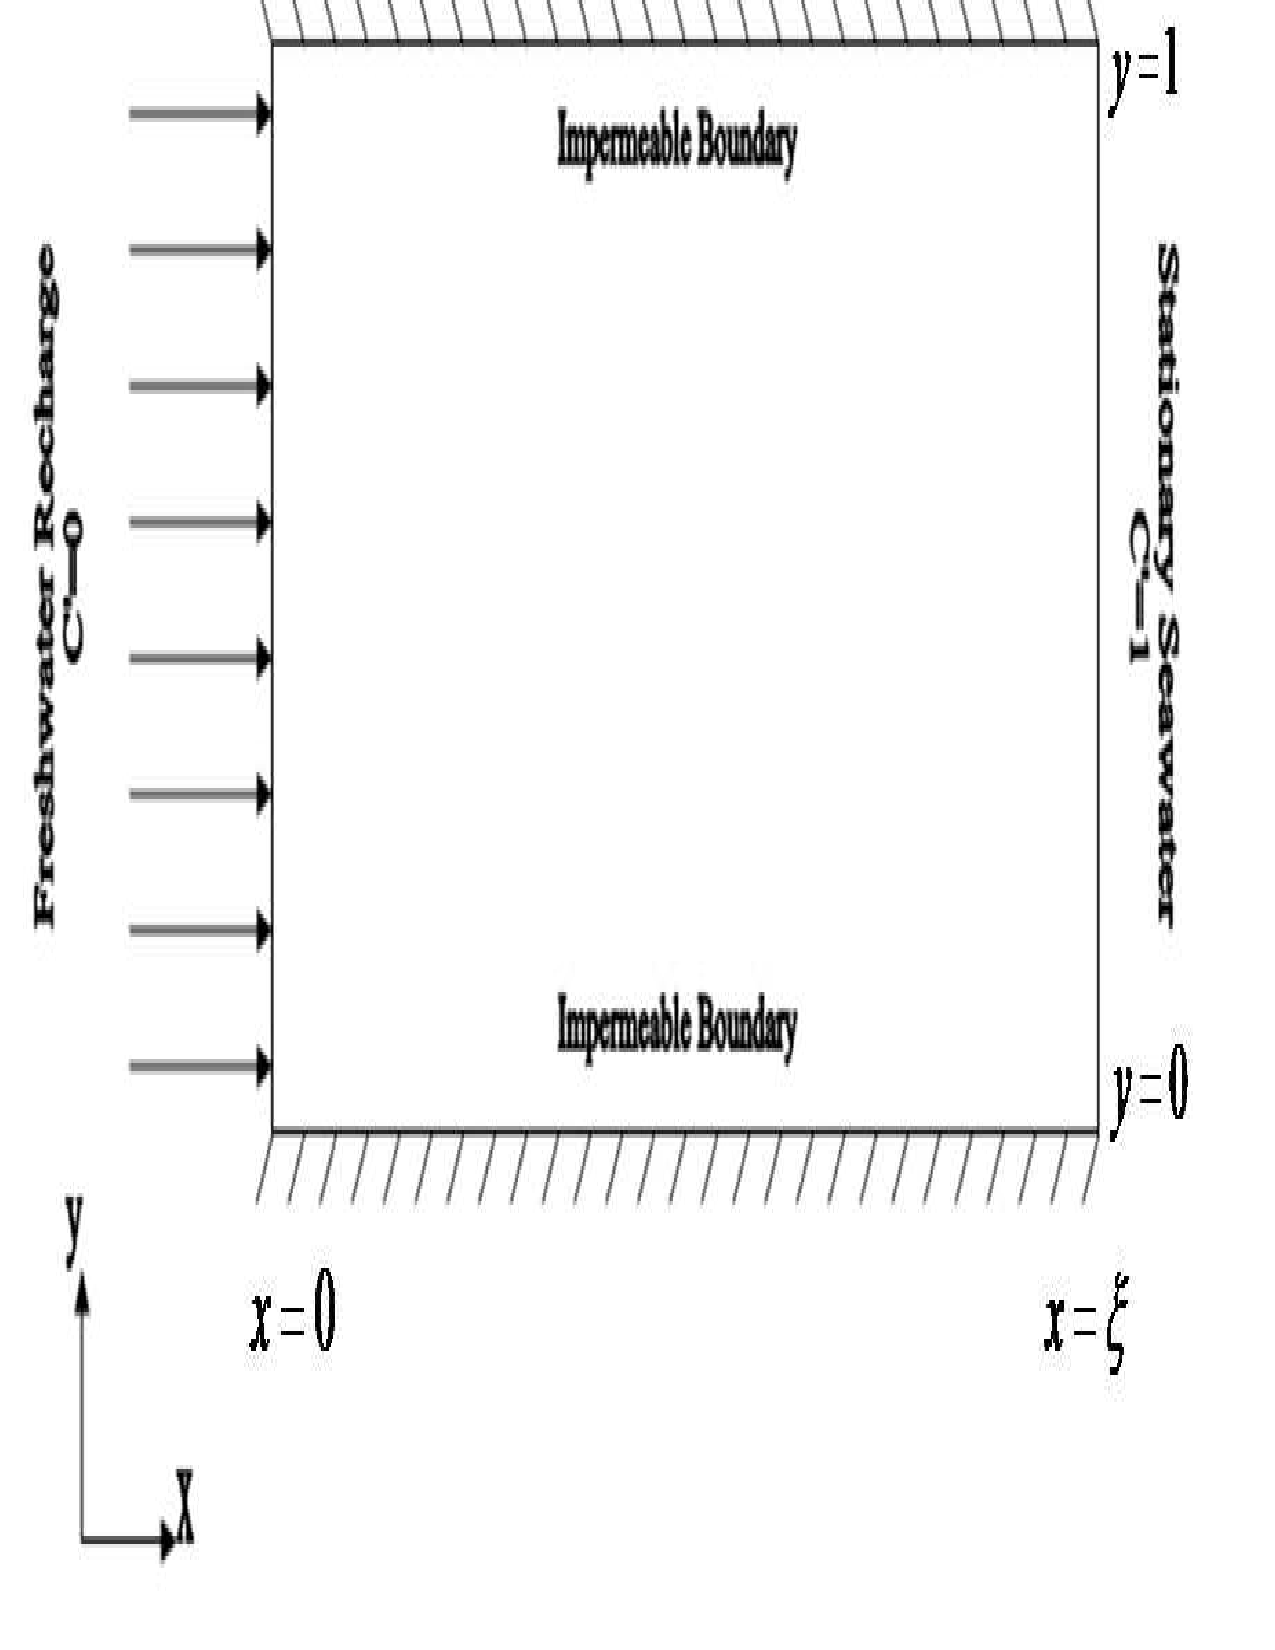
\includegraphics[scale=0.25]
    {image1}
    \caption{Depiction of 2D problem domain} \label{fig:Domain}
\end{figure}

Recently seawater intrusion has become a significant problem in coastal regions.  As populations
increase in these regions, natural recharge no longer counteracts the effects of withdrawals, and so
it is important to have a tool that can estimate the amount of seawater intrusion that may occur
with the continued withdrawal from coastal aquifers. Several numerical models have been developed to
address seawater intrusion in coastal aquifers, and so it is important to have an analytic solution
to use as a benchmark. The benchmarking of numerical code against analytic solutions is a necessary
step in verifying the correctness of the numerical approximations \cite{Simpson}.

Henry's Problem has been widely used as a benchmark case for numerical models of seawater intrusion.
Henry's Semi-Analytic Solution to Seawater Intrusion has been tempered by both the inability to use,
powerful computing technologies, which has become readily available to researchers, and a lack of a
sufficient number of Fourier coefficients, so as to ensure a smooth convergence. In fact, S\'egol
\cite{Segol} suggested that discrepancies between Henry and her own solutions may have been a result
of a lack of convergence in Henry's solution, due to a lack of powerful computing of the time, and
what S\'egol suggests was a poor initial guess. 

The method used by Henry to evaluate his Analytic solution has been plagued by the inability to use
a large number of Fourier coefficients, and therefore does not allow for realistic parameter values
Which have also prevented Henry's Solution from simulating narrow zones of dispersion. This is due
to Henry's method having a substantially low convergences rate with respect to the important
parameters $a$ and $b$.  Since Newton's method has a quadratic rate of convergence for well behaved
problems, one might expect greater ease in calculation for lower values of $a$ and $b$.  Therefore,
Newton's Method would address the convergence issues seen by Henry and others when trying to
simulate narrow zones of dispersion.

Newton's Method not only provides for a previously unused method for solving Henry's Problem, but
will also allow for more Fourier coefficients to be used in the solution, therefore allowing for a
more realistic solution sets. As more terms are used in a Fourier series the closer the numerical
solution comes to the true solution. Using Newton's method allows for the use of any number of
Fourier coefficients, and so it is now possible to evaluate Henry's Semi-Analytic Solution for
narrow zones of dispersion. The improved accuracy and the ability to simulate narrow zones of
dispersion will therefore improve Henry's Problem as a benchmark for comparison to numerical
solutions.

In this paper, we calculate the Fourier coefficients for the Henry problem by using Newton's method
to solve the nonlinear system of equations. Various truncations of the Fourier series are tested and
results are compared against the available result using Henry's method. Finally, $a$ and $b$ are
decreased to more realistic values and results are compared against numerical results from SUTRA
with similar parameter values.


\section{Governing Equations}
Henry's solution considers dispersion of salt into the freshwater, resulting in Darcy's equation
being written with density as a variable. The resulting general vector form of Darcy's equation is

\begin{equation} \label{ZEqnNum283874}
    \stackrel{\rightharpoonup}{q}=-{\raise0.7ex\hbox{\spbox{k} } \!\mathord{\left/
    {\vphantom {k \mu }} \right. \kern-\nulldelimiterspace} \!\lower0.7ex\hbox{$ \mu
    $}} \left(\nabla P-\rho \stackrel{\rightharpoonup}{g} \right) 
\end{equation} 

Continuity equations, such as conservation of the mass of salt and water, must also be satisfied in
addition to equation \eqref{ZEqnNum283874}. The conservation of mass of water in steady flow is
given by,

\begin{equation} \label{ZEqnNum833854} 
    \nabla \cdot \rho _{w}
    \stackrel{\rightharpoonup}{q}=0 
\end{equation} 

where $\rho _{w} $ is the mass per unit volume of pure water. The conservation of the mass of salt
is similar to that of \eqref{ZEqnNum833854} and is given by,

\begin{equation} \label{ZEqnNum750616} 
    \nabla \cdot
    c\stackrel{\rightharpoonup}{q}_{e} =0 
\end{equation} 

where c is the mass per unit volume of salt, and $\stackrel{\rightharpoonup}{q}_{e} $ is the
effective velocity of the movement of salt. This velocity is the result of the sum of the average
fluid velocity $\stackrel{\rightharpoonup}{q}$ and the dispersive movement of salt \cite{Henry60}.
$c\stackrel{\rightharpoonup}{q}_{e} $ is therefore the mass flux of salt, and yields an equation of
the form

\begin{equation} \label{ZEqnNum692228} 
    c\stackrel{\rightharpoonup}{q}_{e} = c\stackrel{\rightharpoonup}{q}-D\nabla c 
\end{equation} 

Taking the divergence of \eqref{ZEqnNum692228} and applying
\eqref{ZEqnNum750616} results in

\begin{equation} 
    \label{ZEqnNum193707} \nabla \cdot
    c\stackrel{\rightharpoonup}{q}-\nabla \cdot D\nabla c=0 
\end{equation} 

For convenience Henry introduced the following dimensionless quantities

\begin{equation} \label{ZEqnNum621601} 
    u'=\frac{ud}{Q} \csp v'=\frac{vd}{Q}
     \csp x'=\frac{x}{d} \csp y'=\frac{y}{d} \csp c'=\frac{c}{c_{s} }
    =\frac{\rho -\rho _{0} }{\rho _{s} -\rho _{0} } 
\end{equation}

Equation \eqref{ZEqnNum833854} was then simplified by using the empirical
relation \cite{Baxter} \cite{Henry60}:
\begin{equation} \label{ZEqnNum679206} 
    \rho =\rho _{w} +c=\rho _{0} + \left(1-E\right)c 
\end{equation} 

where E is a dimensionless constant and is approximately 0.3 for salt concentrations up to that of
seawater \cite{Henry60}. Inserting \eqref{ZEqnNum679206} into \eqref{ZEqnNum833854} yields the new
equation

\begin{equation} \label{ZEqnNum370033} 
    \nabla \cdot \stackrel{\rightharpoonup}{q}-\frac{Ec_{s} }{\rho _{0} } 
    \nabla c'\stackrel{\rightharpoonup}{q}=0 
\end{equation}

In seawater ${c_{s} \mathord{\left/ {\vphantom {c_{s} \rho _{0} }} \right.
\kern-\nulldelimiterspace} \rho _{0} } $ is approximately 0.027 \cite{Henry60}.  Therefore, the
second term in \eqref{ZEqnNum370033} is negligible. This results in a stream function which can be
defined as a dimensionless quantity using the relationships

\begin{equation} \label{ZEqnNum615527} 
    u'=\pderiv{\psi '}{y'} \text{,\; v} '=-\pderiv{\psi '}{x'} 
\end{equation} 

In Equation \eqref{ZEqnNum283874} the pressure term can be eliminated by
rewriting \eqref{ZEqnNum283874} in scalar form:

\begin{equation} \label{ZEqnNum206334} 
    u=-\frac{k}{\mu } \pderiv{P}{x} 
\end{equation}

\begin{equation} \label{ZEqnNum210956} 
    v=-\frac{k}{\mu } \left(\pderiv{P}{y} +\rho g\right) 
\end{equation} 

then differentiating \eqref{ZEqnNum206334} with respect to $y$, and
\eqref{ZEqnNum210956} with respect to $x$ and then subtracting the two. This
results in

\begin{equation} \label{ZEqnNum826101} 
    \pderiv{u}{y} -\pderiv{v}{x} =
    \frac{kg}{\mu } \pderiv{\rho}{x} 
\end{equation}

Converting to a non-dimensional equation by placing \eqref{ZEqnNum621601} into
\eqref{ZEqnNum826101} one obtains

\begin{equation} \label{ZEqnNum965751} 
    \pderiv{u'}{y'}
    -\pderiv{v'}{x'} =\frac{k_{1} d}{Q} \pderiv{c'}{x'} 
\end{equation}

Substituting the relation \eqref{ZEqnNum615527} into \eqref{ZEqnNum965751}
eliminates $\stackrel{\rightharpoonup}{q}$ in favor of $\psi '$ giving:

\begin{equation} \label{ZEqnNum299802} \nabla ^{2} \psi '=\frac{k_{1} d}{Q}
\pderiv{c'}{x'} \end{equation}

In \eqref{ZEqnNum193707} the diffusion coefficient $D$ is a function of velocity, and therefore is
not truly a constant. However, Henry \cite{Henry60} assumed that a ``representative average of the
value of $D$ could be found and used as a constant scalar throughout the field of flow without
distorting the essential features of the problem.'' This assumption will allow for equation
\eqref{ZEqnNum193707} to be written as

\begin{equation} \label{2.15)} \nabla \cdot
c\stackrel{\rightharpoonup}{q}-D\nabla ^{2} c=0 \end{equation}

Now substituting $\psi '\spbox{for} u\spbox{and} v$, and substituting in the relations
from \eqref{ZEqnNum621601} and \eqref{ZEqnNum615527} results in the
dimensionless form

\begin{equation} \label{ZEqnNum195283} 
    \frac{D}{Q} \nabla ^{2} c'=\pderiv{\psi'}{y'} 
    \pderiv{c'}{x'} -\pderiv{\psi'}{x'} 
    \pderiv{c'}{y'} 
\end{equation}

To simplify the equations further Henry introduced the variables 

\begin{equation} \label{ZEqnNum517161} 
    a={Q\mathord{\left/ {\vphantom {Q k_{1} d}} \right. \kern-\nulldelimiterspace} k_{1} d} 
\end{equation}

and 

\begin{equation} \label{ZEqnNum351016} 
    b={D\mathord{\left/ {\vphantom {D Q}} \right. \kern-\nulldelimiterspace} Q} 
\end{equation}

 Substituting \eqref{ZEqnNum517161} and \eqref{ZEqnNum351016} into equations
 \eqref{ZEqnNum299802} and \eqref{ZEqnNum195283}, respectively, resulting in

\begin{equation} \label{2.19)} 
    a\nabla ^{2} \psi '=\pderiv{c'}{x'} 
\end{equation}

and

\begin{equation} \label{2.20)} 
    b\nabla ^{2} c'=\pderiv{\psi'}{y'} \pderiv{c'}{x'} -\pderiv{\psi'}{x'} \pderiv{c'}{y'} 
\end{equation} 

The impermeable boundaries at the top and the bottom of the aquifer require a zero normal velocity
($q_{n} =0$), and so it follows that $\psi '$is a constant at those boundaries. This impermeable
boundary also precludes salt from crossing those boundaries and therefore requires the normal
derivative $\pderiv{c'}{y'} =0$.

The vertical boundaries at the ends of the aquifer, in contact with the freshwater and the seawater
bodies, require $c'=0\spbox{and} c'=1$, respectively.  Also, the hydrostatic pressure distributions
require that $\pderiv{\psi'}{x'} =0$ at both ends of the aquifer. These boundary conditions can be
summarized as follows:

\begin{equation} \label{BC)} \begin{array}{lcr} 
    \psi ' = 0, \pderiv{c'}{y'} =0 \spbox{at} y'=0
    & \qquad
    & \pderiv{\psi'}{x'} = 0, c' = 0 \spbox{at} x'=0 \\
    \psi '= 1, \pderiv{c'}{y'} = 0 \spbox{at} y'=1
    & \qquad
    & \pderiv{\psi'}{x'} =0,  c'=1 \spbox{at} x'=\xi 
\end{array} \end{equation}



%\section{Fourier-Galerkin Method}
%Henry uses a Fourier series to decompose the non-linear differential equations into a sum of
orthogonal basis functions. Then Henry uses what he calls Galerkin's Method to solve for the Fourier
coefficients. In this case Galerkin's Method refers to substituting the Fourier series back into the
differential equations, multiplying both differential equations by orthogonal functions, and then
integrating over the rectangular domain. First, new variables were introduced to further simplify
the boundary conditions. Letting

\begin{equation} \label{3.1)} 
    \Psi = \psi '-y'\csp C = c'-\frac{x'}{\xi } 
\end{equation}

and after dropping the primes, and using subscripts to denote differentiation,
the problem in terms of $\Psi \spbox{and} C$ becomes

\begin{equation} \label{ZEqnNum626661} 
    a\nabla ^{2} \Psi =C_{x} +\frac{1}{\xi } 
\end{equation} 
\begin{equation} \label{ZEqnNum183863} 
    b\nabla ^{2} C=\Psi _{y} C_{x} -\Psi _{x} C_{y} +\frac{1}{\xi } \Psi _{y} +C_{x} +\frac{1}{\xi } 
\end{equation} 
\begin{equation} \label{ZEqnNum529054} 
    C_{y} =0 \csp \Psi =0, \spbox{at} y = 0,1; \quad C = 0\csp \Psi
    _{x} = 0, \spbox{at}x=0,\xi
\end{equation}

$\Psi\spbox{and} C$ can be represented by a double Fourier series that satisfies
\eqref{ZEqnNum529054} \cite{Henry60}

\begin{equation} \label{ZEqnNum807044} \Psi =\sum _{m=1}^{\infty } \sum
_{n=0}^{\infty }A_{m,n} \sin \left(m\pi y\right)\cos \left(n\pi \frac{x}{\xi }
\right) \end{equation}

\begin{equation} \label{ZEqnNum170840} C=\sum _{r=0}^{\infty } \sum
_{s=1}^{\infty }B_{r,s} \cos \left(r\pi y\right)\sin \left(s\pi \frac{x}{\xi }
\right) \end{equation}

Substituting equations \eqref{ZEqnNum807044} and \eqref{ZEqnNum170840} into
\eqref{ZEqnNum626661} and \eqref{ZEqnNum183863}, then multiplying
\eqref{ZEqnNum626661} by $4\sin \left(g\pi y\right)\cos \left(h\pi \frac{x}{\xi
} \right)$, and multiplying \eqref{ZEqnNum183863} by $4\cos \left(g\pi
y\right)\sin \left(h\pi \frac{x}{\xi } \right)$ integrating over the rectangular
domain, results in a few different integrals to be evaluated. But, before
evaluating any integral one should first realize two things; first,

\begin{equation} \label{3.7)} \sin (g\pi )=0 \quad \forall g\in {\mathbb Z}
\end{equation}
and second, 
\begin{equation} \label{ZEqnNum821421} \cos \left(h\pi \right)\equiv
\left(-1\right)^{h} \quad \forall h\in {\mathbb Z} \end{equation}

These two facts will come in very handy when simplifying the result of each
integral. 

For simplicity it will be easier to evaluate each integral separately, rather
than to treat the entire equation all at once. The left hand side of equation
\eqref{ZEqnNum626661} becomes

\begin{equation} \label{ZEqnNum923088} \begin{split} 
    a \pi ^{2} \sum _{m=1}^{\infty} \sum_{n=0}^{\infty} 
    & \left(m^{2} + \frac{n^{2}}{\xi ^{2}} \right) A_{m,n} \cdot \\
    & \int _{0}^{1} \int _{0}^{\xi} 4 \sin \left(g \pi y \right) 
    \sin \left(m\pi y\right) \cos \left(n \pi \frac{x}{\xi} \right)
    \cos \left(h \pi \frac{x}{\xi} \right) dxdy  
\end{split} \end{equation}

The right hand side of equation \eqref{ZEqnNum626661} will be split into two
parts, $C_{x} \spbox{and} \frac{1}{\xi } $, in which one obtains
\begin{equation} \label{ZEqnNum851626} \begin{split}
    \frac{\pi}{\xi} \sum _{r=0}^{\infty} \sum _{s=1}^{\infty}  
    & B_{r,s} \cdot s \cdot \\
    & \int_{0}^{1} \int _{0}^{\xi } 4 \sin \left(g \pi y\right) 
    \cos (r\pi y)\cos \left(h\pi \frac{x}{\xi} \right)\cos
    \left(s\pi \frac{x}{\xi} \right) dxdy  
\end{split} \end{equation}
and
\begin{equation} \label{ZEqnNum379567} \frac{1}{\xi } \int _{0}^{1} \int
_{0}^{\xi }4\sin \left(g\pi y\right)\cos \left(h\pi \frac{x}{\xi } \right)dxdy
\end{equation}
respectively.

Beginning with the simplest integral first, which is of course
\eqref{ZEqnNum379567}. First, notice that if $h\ne 0$ then the entire integral
will be zero. Integral \eqref{ZEqnNum379567} when evaluated using the above
observation becomes
\begin{equation*}
    \frac{1}{\xi } \int _{0}^{1} \int _{0}^{\xi }4\sin \left(g\pi y\right)dxdy
    =\frac{4}{\pi } \frac{1-\cos \left(g\pi \right)}{g} 
\end{equation*}

Using relationship \eqref{ZEqnNum821421} one obtains the result

\begin{equation*}
    \frac{1}{\xi } \int _{0}^{1} \int _{0}^{\xi }4\sin \left(g\pi y\right)dxdy
    \equiv \frac{1-\left(-1\right)^{g} }{g} 
\end{equation*}

and using the observation, if $g = 0$ then the entire integral will evaluate to
zero, and therefore integral \eqref{ZEqnNum379567} becomes

\begin{equation} \label{ZEqnNum309765} 
    \frac{1}{\xi } \int _{0}^{1} \int _{0}^{\xi } 4 \sin \left(g\pi y\right) 
    \cos \left(h\pi \frac{x}{\xi } \right)dxdy
    =\frac{4}{\pi } W\left(g,h\right) 
\end{equation}

where

\begin{equation}\label{3.13} 
    \ctfunc{W\left(g,h\right)}
    {0}{\text{for } h \ne 0}
    {0}{\text{for } g = 0}
    {\frac{1 - \left(-1 \right)^{g}}{g}}{\text{for } h = 0}. 
\end{equation}

When finishing the right hand side of equation \eqref{ZEqnNum626661} one should
notice the integral \eqref{ZEqnNum851626} will only be non-zero when $s=h$. This
results in \eqref{ZEqnNum851626} becoming

\begin{equation} \label{ZEqnNum929872} 
    \frac{\pi }{\xi } \sum _{r=0}^{\infty} B_{r,h} \cdot 
    h\int _{0}^{1} \int _{0}^{\xi} 4\sin \left(g\pi y\right)
    \cos (r \pi y)\cos ^{2} \left(h\pi \frac{x}{\xi } \right) dxdy 
\end{equation}

Using the double angle formula $\cos ^{2} x=\frac{\cos \left(2x\right)+1}{2} $,
and substituting this into \eqref{ZEqnNum929872}, one obtains

\begin{equation} \label{ZEqnNum253937} 
    \frac{\pi }{\xi } \sum _{r=0}^{\infty} B_{r,h} \cdot 
    h \int _{0}^{1}2\sin \left(g\pi y\right)\cos (r\pi y) 
    \int_{0}^{\xi } \left(\cos \left(2h\pi \frac{x}{\xi } \right) + 1 \right) dxdy
\end{equation}

Simplifying the integral further one uses the relation $2\sin \left(x\right)\cos
\left(y\right)=\sin \left(x+y\right)+\sin \left(x-y\right)$,
\eqref{ZEqnNum253937} becomes

\begin{equation} \label{ZEqnNum322465} \begin{split}
    \frac{\pi }{\xi } \sum _{r=0}^{\infty} B_{r,h} \cdot 
    & h\int _{0}^{1} \left( \sin \left[ \left( g + r \right) \pi y \right] + 
    \sin \left[ \left(g - r\right) \pi y \right] \right) \cdot \\
    & \int _{0}^{\xi} \left(\cos \left(2h\pi \frac{x}{\xi} \right) + 1\right) dxdy 
\end{split} \end{equation} 

To evaluate this integral, first look at the integral $\int _{0}^{\xi} 
\left(\cos \left(2h\pi \frac{x}{\xi } \right)+1\right) dx$. Evaluating this
integral one obtains

\begin{equation} \label{ZEqnNum494103} \int _{0}^{\xi } \left(\cos \left(2h\pi
\frac{x}{\xi } \right)+1\right) dx=\xi \end{equation}

Substituting \eqref{ZEqnNum494103} into \eqref{ZEqnNum322465} one obtains

\begin{equation} \label{ZEqnNum504644} \pi \sum _{r=0}^{\infty }B_{r,h} \cdot
h\int _{0}^{1} \left(\sin \left[\left(g+r\right)\pi y\right]+\sin
\left[\left(g-r\right)\pi y\right]\right) dy \end{equation}

Evaluating the integral $\pi \int _{0}^{1} \left(\sin \left[\left(g+r\right)\pi
y\right]+\sin \left[\left(g-r\right)\pi y\right]\right) dy$ results in

\begin{equation*} \begin{split}
    \pi \int _{0}^{1} \sin \left[\left(g + r\right)\pi y\right]
    & + \sin \left[\left(g - r\right) \pi y\right] dy \\
    & = \frac{\cos \left[\left(g + r\right)\pi \right] - 1}{g + r} 
    + \frac{\cos \left[\left(g - r \right) \pi \right] - 1}{g - r} 
\end{split} \end{equation*} 

Using the relationship \eqref{ZEqnNum821421} one obtains

\begin{equation*}
    \pi \int _{0}^{1} \left(\sin \left[\left(g+r\right)\pi y\right]+\sin
    \left[\left(g-r\right)\pi y\right]\right) dy\equiv \frac{\left(-1\right)^{g+r}
    -1}{g+r} +\frac{\left(-1\right)^{g-r} -1}{g-r} 
\end{equation*}

One should notice that this becomes undefined if $r=g$, and so one must evaluate
the integral for when $r=g$. When $r=g$ the integral becomes

\begin{equation*}
    \pi \int _{0}^{1} \sin \left(2g\pi y\right) dy = 0
\end{equation*} 

 Therefore the integral \eqref{ZEqnNum504644} becomes

\begin{equation*}
    \pi \sum _{r=0}^{\infty }B_{r,h} \cdot h\int _{0}^{1} \left(\sin
\left[\left(g+r\right)\pi y\right]+\sin \left[\left(g-r\right)\pi
y\right]\right) dy =\sum _{r=0}^{\infty }B_{r,h} \cdot h\cdot N\left(g,r\right)
\end{equation*}

where

\begin{equation} \label{3.19)} 
    N\left(g,r\right) = \begin{cases}
    0 & \text{for } r = g \\
    \frac{\left(-1\right)^{g + r} - 1}{g + r} + \frac{\left(-1\right)^{g - r} - 1}{g - r} 
    & \text{otherwise}\end{cases} 
\end{equation}

 To finish up with \eqref{ZEqnNum626661} integral \eqref{ZEqnNum923088} must be
 evaluated. One should notice that this integral is non-zero only when $m = g
 \spbox{and} n = h$, and therefore \eqref{ZEqnNum923088} becomes

\begin{equation} \label{ZEqnNum599031} 
    a \pi ^{2} \left(g^{2} + \frac{h^{2}}{\xi^{2}} \right)
    A_{g,h} \int _{0}^{1} \int _{0}^{\xi} 4 \sin ^{2} 
    \left(g \pi y\right) \cos ^{2} \left(h \pi \frac{x}{\xi} \right)dxdy 
\end{equation}

Using the double angle formulas, $\cos ^{2} x = \frac{\cos \left(2x\right) + 1}{2} $
and $\sin ^{2} x = \frac{1 - \cos \left(2 x \right)}{2} $, the integral
\eqref{ZEqnNum599031} becomes

\begin{equation} \label{3.21)} 
    a\pi ^{2} \left(g^{2} +\frac{h^{2} }{\xi ^{2} } \right)
    A_{g,h} \int _{0}^{1} \left(1-\cos \left(2g\pi y\right)\right)
    \int_{0}^{\xi } \left(\cos \left(2h \pi \frac{x}{\xi } \right) + 1\right) dxdy
\end{equation}

Since $h$ can be zero, one must evaluate this integral for the two cases
$h = 0 \spbox{and} h \ne 0$, resulting in

\begin{equation} \label{3.22)} 
    \begin{array}{l} {a\pi ^{2} \left(g^{2}
    +\frac{h^{2} }{\xi ^{2} } \right)A_{g,h} \int _{0}^{1} \left(1-\cos \left(2g\pi
    y\right)\right)\int _{0}^{\xi } \left(\cos \left(2h\pi \frac{x}{\xi }
    \right)+1\right)dxdy } \\ {=\varepsilon \left(h\right)\cdot a\pi ^{2}
    \left(g^{2} +\frac{h^{2} }{\xi ^{2} } \right)A_{g,h} \cdot \xi } \end{array}
\end{equation}

where

\begin{equation} \label{3.23)} 
    \varepsilon \left(h\right) = \begin{cases}
        2 & h = 0 \\ 
        1 & \text{otherwise}\end{cases} 
\end{equation} 

The more complex equation \eqref{ZEqnNum183863} will have to be dealt with in
several parts. First, the left hand side of equation \eqref{ZEqnNum183863}
becomes

\begin{equation} \label{ZEqnNum189325} \begin{split} 
    b\pi ^{2} \sum _{r=0}^{\infty } \sum_{s=1}^{\infty } 
    & \left(r^{2} + \frac{s^{2} }{\xi^{2} } \right) B_{r,s} \\ 
    & \int_{0}^{1} \int_{0}^{\xi } 4 \cos \left(g \pi y\right) 
    \cos \left(r\pi y\right) \sin\left(s \pi \frac{x}{\xi} \right)
    \sin \left(h \pi \frac{x}{\xi} \right) dxdy
\end{split} \end{equation}

 To deal with the right hand side of the equation it will be much simpler to
 split it into its separate derivatives. However, grouping the derivatives $\Psi
 _{y} C_{x} \spbox{and} \Psi _{x} C_{y} $ will be convenient later. The derivatives
 $\Psi _{y} C_{x} \spbox{and} \Psi _{x} C_{y} $ result in

\begin{equation} \label{ZEqnNum757716} \begin{array}{l} {\Psi _{y} C_{x} -\Psi
_{x} C_{y} =} \\ {\frac{\pi }{\xi } ^{2} \sum _{m=1}^{\infty } \sum
_{n=0}^{\infty } \sum _{r=0}^{\infty } \sum _{s=1}^{\infty }A_{m,n} B_{r,s}
[ms\int _{0}^{1} \int _{0}^{\xi }4\cos \left(g\pi y\right)\cos \left(m\pi
y\right)\cos \left(r\pi y\right) } \\ {\cdot \sin \left(h\pi \frac{x}{\xi}
\right)\cos \left(n\pi \frac{x}{\xi } \right)\cos \left(s\pi \frac{x}{\xi }
\right)dxdy} \\ {-nr\int _{0}^{1} \int _{0}^{\xi }4\cos \left(g\pi y\right)\sin
\left(m\pi y\right)\sin \left(r\pi y\right)} \\ {\sin \left(h\pi \frac{x}{\xi }
\right)\sin \left(n\pi \frac{x}{\xi } \right)\sin \left(s\pi \frac{x}{\xi }
\right)dxdy]} \end{array} \end{equation}

For the portion of the right hand side of equation \eqref{ZEqnNum183863}
represented by $\frac{1}{\xi } \Psi _{y} $ one obtains

\begin{equation} \label{ZEqnNum659914} \frac{\pi }{\xi } \sum _{m=1}^{\infty
} \sum _{n=0}^{\infty }A_{m,n} \cdot m\int _{0}^{1} \int _{0}^{\xi }4\cos
\left(g\pi y\right)\cos \left(m\pi y\right)\sin \left(h\pi \frac{x}{\xi }
\right)\sin \left(n\pi \frac{x}{\xi } \right) dxdy \end{equation}

The treatment of the terms $C_{x} \spbox{and} \frac{1}{\xi } $ in
\eqref{ZEqnNum183863}, is very similar to those of the right hand side of
equation \eqref{ZEqnNum626661}. Galerkin's Method should result in $C_{x} {\rm
\; and\; } \frac{1}{\xi } $ becoming

\begin{equation} \label{ZEqnNum392315} \frac{\pi }{\xi } \sum _{r=0}^{\infty
} \sum _{s=1}^{\infty } \left[B_{r,s} \cdot s\int _{0}^{1} \int _{0}^{\xi }4\cos
\left(g\pi y\right)\cos (r\pi y)\sin \left(h\pi \frac{x}{\xi } \right)\cos
\left(s\pi \frac{x}{\xi } \right)dxdy \right] \end{equation}s

and

\begin{equation} \label{ZEqnNum600143} \frac{1}{\xi } \int _{0}^{1} \int
_{0}^{\xi }4\cos \left(g\pi y\right)\sin \left(h\pi \frac{x}{\xi } \right)dxdy
\end{equation} 

respectively. In fact, the difference between integrals \eqref{ZEqnNum379567}
and \eqref{ZEqnNum600143} consists in $x\spbox{and}y$ switching positions.
So the result obtained from \eqref{ZEqnNum309765} can then be applied to
integral \eqref{ZEqnNum600143}. Therefore, one obtains

\begin{equation} \label{3.29)} \frac{1}{\xi } \int _{0}^{1} \int _{0}^{\xi }4\cos
\left(g\pi y\right)\sin \left(h\pi \frac{x}{\xi } \right)dxdy =\frac{4}{\pi }
W\left(h,g\right) \end{equation}

 The integral \eqref{ZEqnNum392315}, as stated before, is very similar to the
 integral \eqref{ZEqnNum851626}. In fact, the difference between integral
 \eqref{ZEqnNum392315} and integral \eqref{ZEqnNum851626} is that for
 \eqref{ZEqnNum392315} to be non-zero $r \text{ must\; equal\; } g$ instead of
 $s$equaling $h$, so it is as if the variables have been switched. One
 significant difference is that one must consider when $g=0$, resulting in

\begin{equation} \label{3.30)} \frac{\pi }{\xi } \sum _{r=0}^{\infty } \sum
_{s=1}^{\infty } \left[B_{r,s} \cdot s\int _{0}^{1} \int _{0}^{\xi }4\cos
\left(g\pi y\right)\cos (r\pi y)\sin \left(h\pi \frac{x}{\xi } \right)\cos
\left(s\pi \frac{x}{\xi } \right)dxdy \right] =\varepsilon \left(g\right)\cdot
\sum _{s=1}^{\infty }B_{g,s} \cdot s\cdot N\left(h,s\right) \end{equation}

The integral \eqref{ZEqnNum659914} is also very similar to that of
\eqref{ZEqnNum851626}, differing in that for \eqref{ZEqnNum659914} to be
non-zero, $m \text{ must\; equal\; } g$, resulting in

\begin{equation} \label{3.31)} \frac{\pi }{\xi } \sum _{n=0}^{\infty }A_{g,n}
\cdot g\int _{0}^{1}4\cos ^{2} \left(g\pi y\right)\int _{0}^{\xi } \sin
\left(h\pi \frac{x}{\xi } \right)\sin \left(n\pi \frac{x}{\xi } \right) dxdy
\end{equation}

By similar steps taken to evaluate \eqref{ZEqnNum929872}, one obtains

\begin{equation} \label{3.32)} \frac{\pi }{\xi } \sum _{n=0}^{\infty }A_{g,n}
\cdot g\int _{0}^{1}4\cos ^{2} \left(g\pi y\right)\int _{0}^{\xi } \sin
\left(h\pi \frac{x}{\xi } \right)\sin \left(n\pi \frac{x}{\xi } \right)
dxdy=\sum _{n=0}^{\infty }A_{g,n} \cdot g\cdot N\left(h,n\right) \end{equation} 



For \eqref{ZEqnNum757716} it will much easier to look at each integral
separately. First, look at the integral

\begin{equation*}
    \int _{0}^{1} \int _{0}^{\xi }4\cos \left(g\pi y\right)\cos \left(m\pi
    y\right)\cos \left(r\pi y\right)\sin \left(h\pi \frac{x}{\xi } \right)\cos
    \left(n\pi \frac{x}{\xi } \right)\cos \left(s\pi \frac{x}{\xi } \right)dxdy 
\end{equation*}

Using the relation

\begin{equation*} \begin{split}
    \sin \left(h\pi \frac{x}{\xi } \right)\cos \left(n\pi
    \frac{x}{\xi } \right)\cos \left(s\pi \frac{x}{\xi } \right) 
    & = \sin \left[\left(h+n+s\right)\pi \frac{x}{\xi } \right]
    + \sin \left[\left(h+n-s\right)\pi \frac{x}{\xi } \right] \\ 
    & + \sin \left[\left(h-n+s\right)\pi \frac{x}{\xi } \right]
    +\sin \left[\left(h-n-s\right)\pi \frac{x}{\xi } \right]  
\end{split} \end{equation*}

the integral becomes

\begin{equation*} \begin{split}
    \int _{0}^{1} 4 \cos \left(g \pi y\right) \cos \left(m \pi y\right)
    \cos \left(r \pi y\right) \int _{0}^{\xi } 
    &\sin \left[\left(h + n + s\right) \pi \frac{x}{\xi } \right]
    +\sin \left[\left(h+n-s\right)\pi \frac{x}{\xi } \right] \\ 
    & + \sin \left[\left(h - n + s\right)\pi \frac{x}{\xi } \right] 
    + \sin \left[\left(h - n - s\right)\pi \frac{x}{\xi } \right] dxdy 
\end{split} \end{equation*}

This then simplifies, using the relation \eqref{ZEqnNum821421}, to

\begin{equation*}
    \int _{0}^{1} 4\cos \left(g\pi y\right) 
    \cos \left(m\pi y\right)\cos \left(r \pi y\right)\cdot R dy 
\end{equation*}

Where

\begin{equation} \label{ZEqnNum244131} 
    \cfunc{R}
    {0}{h = n + s \csp h = n - s, \spbox{or} h = s - n}
    {\frac{\left(-1\right)^{h + n + s} - 1}{h + n + s} 
        + \frac{\left(-1\right)^{h + n - s} - 1}{h + n - s}
        + \frac{\left(-1\right)^{h - n + s} - 1}{h - n + s} 
        + \frac{\left(-1\right)^{h - n - s} - 1}{h - n - s}} 
    {\text{otherwise}}
\end{equation}

Then using the relation

\begin{equation*}
    \begin{array}{l} {\cos \left(g\pi y\right)\cos \left(m\pi y\right)\cos
    \left(r\pi y\right)=\cos \left[\left(g+m+r\right)\pi y\right]+\cos
    \left[\left(g+m-r\right)\pi y\right]} \\ {+\cos \left[\left(g-m+r\right)\pi
    y\right]+\cos \left[\left(g-m-r\right)\pi y\right]} \end{array} 
\end{equation*}

The integral now becomes 
\begin{equation*} \begin{split}
    \int_{0}^{1} 4(\cos \left[\left(g + m + r\right) \pi y\right]
    & + \cos \left[\left(g + m - r\right)\pi y\right] \\
    & + \cos \left[\left(g - m + r\right)\pi y\right]
    + \cos \left[\left(g - m - r\right)\pi y\right] ) Rdy 
\end{split} \end{equation*}
This integral is non-zero only when $g = m - r \csp 
g = r - m \text{, or when } g = m + r$. Using these facts to evaluate the previous
integral results in

\begin{equation*} \begin{split}
    \int _{0}^{1} 4 (\cos \left[\left(g + m + r\right)\pi y\right]
    & + \cos \left[\left(g + m - r\right) \pi y\right] \\
    & + \cos \left[\left(g - m + r\right) \pi y\right]
    + \cos \left[\left(g - m - r\right) \pi y\right] ) R dy = LR
\end{split} \end{equation*} 

where

\begin{equation} \label{ZEqnNum236446} L=\delta _{\left(m-r\right),g} +\delta
_{\left(r-m\right),g} +\delta _{\left(m+r\right),g} \end{equation}

The $\delta $ used in \eqref{ZEqnNum236446} is the Kronecker delta:

\begin{equation*}
    \cfunc{\delta _{i,j}}
    {0}{i \ne j}
    {1}{i = j}
\end{equation*}

Similarly the second portion of the integral \eqref{ZEqnNum757716} can be
evaluated in a very similar fashion resulting in

\begin{equation*}
    \int _{0}^{1} \int _{0}^{\xi} 4 \cos \left(g\pi y\right)
    \sin \left(m \pi y\right) \sin \left(r \pi y\right) 
    \sin \left(h \pi \frac{x}{\xi } \right)
    \sin \left(n \pi \frac{x}{\xi } \right)
    \sin \left(s\pi \frac{x}{\xi } \right) dxdy
    = FG
\end{equation*}

where
\begin{equation} \label{ZEqnNum668374} 
    \cfunc{G}
    {0}{\begin{array}{l} 
        h = n + s \csp h = n - s, \\ 
        \spbox{or} h = s - n
    \end{array}}
    {\begin{array}{ll} 
        \frac{\left(-1\right)^{h + n + s} - 1}{h + n + s}  
       + & \frac{\left(-1\right)^{h + n - s} - 1}{h + n - s} \\
       & - \frac{\left(-1\right)^{h - n + s} - 1}{h - n + s} 
        - \frac{\left(-1\right)^{h - n - s} - 1}{h - n - s}
    \end{array}}{\text{otherwise}} 
\end{equation}

and
\begin{equation} \label{3.36)} 
    F = \delta _{\left(m-r\right),g} 
    + \delta_{\left(r-m\right),g} - \delta _{\left(m + r\right), g} 
\end{equation}

Combining the two parts of \eqref{ZEqnNum757716} results in

\begin{equation} \label{3.37)} \begin{split} 
    & \frac{\pi }{\xi } ^{2} 
    \sum_{m=1}^{\infty } \sum _{n=0}^{\infty } \sum _{r=0}^{\infty } \sum _{s=1}^{\infty}
        A_{m,n} B_{r,s} m s \\
        & \int _{0}^{1} \int _{0}^{\xi} 4\cos \left(g \pi y\right) \cos \left(m\pi y\right)
            \cos \left(r\pi y\right) \cdot \sin \left( h\pi \frac{x}{\xi } \right)
            \cos \left(n\pi \frac{x}{\xi } \right)
            \cos \left(s\pi \frac{x}{\xi } \right) dxdy \\ 
        & - nr \int_{0}^{1} \int_{0}^{\xi} 4 \cos \left(g \pi y\right) \sin \left(m\pi y\right) 
            \sin \left(r \pi y\right) \sin \left(h\pi \frac{x}{\xi} \right) 
            \sin \left(n\pi \frac{x}{\xi } \right) \sin \left(s\pi \frac{x}{\xi} \right) dxdy \\
    & = \frac{\pi}{4} \sum _{m = 1}^{\infty} \sum_{n=0}^{\infty } \sum _{r=0}^{\infty } \sum _{s=1}^{\infty } 
        A_{m,n} B_{r,s} \left(msLR - nrFG\right)
\end{split} \end{equation} 

To finish equation \eqref{ZEqnNum183863}, the left hand side, the integral \eqref{ZEqnNum189325},
must be evaluated. It should be easy to see that the results are very similar to that of the
evaluation of the left hand side of equation \eqref{ZEqnNum626661}, that is the integral
\eqref{ZEqnNum923088}. And so, the evaluation of \eqref{ZEqnNum189325} results in

\begin{equation} \label{3.38)} \begin{array}{l} 
    b \pi ^{2} \sum _{r=0}^{\infty} \sum _{s=1}^{\infty } 
        \left[\left(r^{2} + \frac{s^{2} }{\xi ^{2} } \right) 
        B_{r,s} \int _{0}^{1} \int _{0}^{\xi } 
        4 \cos \left(g\pi y\right) \cos \left(r \pi y\right)
        \sin \left(s\pi \frac{x}{\xi} \right)
        \sin \left(h\pi \frac{x}{\xi} \right) dxdy \right] \\ 
    = \varepsilon (g)b\pi ^{2} B_{g,h} \left(g^{2}
        +\frac{h^{2} }{\xi ^{2} } \right)\xi
\end{array} \end{equation}

Putting all these results together one will arrive at

\begin{equation} \label{ZEqnNum704007} 
    \varepsilon \left(h\right)\cdot a \pi ^{2} A_{g,h} \left(g^{2} 
    + \frac{h^{2} }{\xi ^{2} } \right) \xi 
    = \sum _{r=0}^{\infty} B_{r,h} \cdot h \cdot N \left(g,r\right) 
    + \frac{4}{\pi} W \left(g, h\right)
\end{equation}

\begin{equation} \label{ZEqnNum765213} 
    \begin{array}{l} 
    \varepsilon \left(g\right) \cdot b \pi ^{2} B_{g,h} 
    \left(g^{2} + \frac{h^{2}}{\xi ^{2}}\right) \xi 
    = \frac{\pi }{4} 
    \sum _{m=1}^{\infty } \sum _{n=0}^{\infty } \sum_{r=0}^{\infty } \sum _{s=1}^{\infty}
    A_{m,n} B_{r,s} \left(msLR - nrFG\right) \\
    + \sum _{n=0}^{\infty} A_{g,n} \cdot g \cdot N \left(h, n\right) 
    + \varepsilon \left(g \right) \cdot \sum _{s=1}^{\infty} B_{g,s} 
    \cdot s\cdot N\left(h, s\right) + \frac{4}{\pi } W\left(g,h\right)
\end{array} \end{equation}

The notation used in equations \eqref{ZEqnNum704007} and \eqref{ZEqnNum765213}
have been defined below:

\begin{equation*}
    F = \delta _{\left(m - r\right), g} + \delta _{\left(r - m\right), g} - 
    \delta _{\left(m + r\right), g}
\end{equation*}

\begin{equation*}
    L=\delta _{\left(m - r\right), g} +\delta _{\left(r - m\right), g} + \delta
    _{\left(m + r\right), g} 
\end{equation*}

\begin{equation} \label{ZEqnNum668374} 
    \cfunc{G}
    {0}{\begin{array}{l} 
        h = n + s \csp h = n - s, \\ 
        \spbox{or} h = s - n
    \end{array}}
    {\begin{array}{ll} 
        \frac{\left(-1\right)^{h + n + s} - 1}{h + n + s}  
       + & \frac{\left(-1\right)^{h + n - s} - 1}{h + n - s} \\
       & - \frac{\left(-1\right)^{h - n + s} - 1}{h - n + s} 
        - \frac{\left(-1\right)^{h - n - s} - 1}{h - n - s}
    \end{array}}{\text{otherwise}} 
\end{equation}

\begin{equation*}
    \cfunc{R}
    {0}
    {h = n + s \csp h = n - s \spbox{or} h = s - n}
    {\frac{\left(-1\right)^{h + n + s} - 1}{h + n + s} +
    \frac{\left(-1\right)^{h + n - s} - 1}{h + n - s} + 
    \frac{\left(-1\right)^{h - n + s} - 1}{h - n + s} + 
    \frac{\left(-1\right)^{h - n - s} - 1}{h - n - s}}
    { \text{otherwise}}  
\end{equation*}

\begin{equation*}
    \cfunc{N\left(g,r\right)}
    {0}
    {r = g}
    {\frac{\left(-1\right)^{g + r} - 1}{g + r} + 
    \frac{\left(-1\right)^{g - r} - 1}{g - r}} 
    {otherwise} 
\end{equation*}

\begin{equation*}
    \ctfunc{W\left(g,h\right)}
    {0}
    {h \ne 0}
    {0}
    {g=0}
    {\frac{1 - \left(-1\right)^{g} }{g} }
    {h = 0}
\end{equation*}

\begin{equation*}
    \cfunc{\delta _{i,j} }
    {0}
    {i \ne j}
    {1}
    {i = j}
\end{equation*}

\begin{equation*}
    \cfunc{\varepsilon \left(g\right)}
    {2}
    {g = 0}
    {1}
    { \text{otherwise}}
\end{equation*}

For one to evaluate this numerically one must truncate the summations, since infinite sums cannot be
evaluated by computational methods. Therefore, an approximation to the true solution will be
obtained using the truncated versions of \eqref{ZEqnNum704007} and \eqref{ZEqnNum765213}.


\section{Newton-Raphson Formulation}
To improve the results obtained by Henry's Analytic solution a Newton-Raphson Method was used.
Originally Henry used a method simple method of linearization, which will be discussed in depth
later. The method originally used by Henry will be discussed in depth later. For Newton's Method to
make sense, in the contexts of Henry's Problem, it is necessary to define a vector $X$ made up of
vectors $A \spbox{and} B$, therefore let

\begin{equation} \label{4.1)} 
    X = \begin{bmatrix}
    A_{1,0} \\ 
    A_{1,1} \\ 
    \vdots \\ 
    A_{i_{a} ,j_{a} } \\ 
    B_{0,1} \\ 
    B_{0,2} \\ 
    \vdots \\
    B_{i_{b} ,j_{b} } \end{bmatrix} \; 
    i_{a} \csp i_{b} \csp j_{a} \csp j_{b} \in \mathbb{Z}^{+} 
\end{equation}

It is also necessary to define a vector function based upon
\eqref{ZEqnNum704007} and \eqref{ZEqnNum765213}, where

\begin{equation} \label{4.2)} 
    \phi _{g,h} \left(X\right) = \varepsilon \left(h \right) a \pi ^{2} 
    \cdot A_{g,h} \cdot \left(g^{2} + \frac{h^{2} }{\xi ^{2}} \right)
    \xi - \sum _{r=0}^{i_{b} }B_{r,h} \cdot h \cdot N\left(g,r\right)
    - \frac{4}{\pi } W\left(g,h\right) 
\end{equation} 
and
\begin{equation} \label{4.3)} \begin{array}{l} 
    \gamma _{g,h} \left(X\right) = \varepsilon \left(g \right) b \pi ^{2} 
    \cdot B_{g,h} \cdot \left(g^{2} + \frac{h^{2}}{\xi ^{2}} \right) \xi 
    - \sum _{n=0}^{i_{a} }A_{g,n} \cdot g \cdot N\left(h,n\right) \\ 
    - \varepsilon \left(g\right) \sum_{s=1}^{i_{b}} 
    B_{g,s} \cdot s \cdot N\left(h,s\right) - \frac{\pi}{4} 
    \sum_{m=1}^{i_{a}} \sum _{n=0}^{j_{a} } \sum _{r=0}^{i_{b}} \sum _{s=1}^{j_{b}} 
    A_{m,n} B_{r,s} \left(msLR - nrFG\right) - \frac{4}{\pi} W\left(h,g\right)
\end{array} \end{equation}

Newton's Method however, takes only one function and therefore these two vector
functions must be combined to make one new vector function. We solve it as a
system and combine both of the above functions in one vector:

\begin{equation} \label{ZEqnNum407215} \Phi
\left(X\right)=\left[\begin{array}{c} {\phi \left(X\right)} \\ {\gamma
\left(X\right)} \end{array} \right] \end{equation}

Let $X^{(n+1)} $be the value of $X$ at the $n+1^{th} $ iteration of the
Multi-Variate Newton-Raphson's Method. We then can write Newton's Method as

\begin{equation} \label{4.5)} X^{\left(n+1\right)} =X^{\left(n\right)} -D\Phi
^{-1} \left(X^{\left(n\right)} \right)\cdot \Phi \left(X^{\left(n\right)}
\right), \text{ \; \; } n\in {\mathbb N} \end{equation}

where $D\Phi \left(X^{\left(n\right)} \right)$ is the Jacobian matrix evaluated
at $X^{\left(n\right)} \spbox{and} D\Phi ^{-1} \left(X^{\left(n\right)} \right)$ is
the inverse to $D\Phi \left(X^{\left(n\right)} \right)$.

For simplicity let $\Phi ^{\left(n\right)} \spbox{denote} \Phi
\left(X^{\left(n\right)} \right)$, $\phi ^{\left(n\right)} {\rm \; denote\;
} \phi \left(X^{\left(n\right)} \right)$, $\gamma ^{\left(n\right)} {\rm \;
denote\; } \gamma \left(X^{\left(n\right)} \right)$, $D\Phi ^{\left(n\right)}
\spbox{denote}D\Phi \left(X^{\left(n\right)} \right)$, and $D\Phi
_{\left(n\right)}^{-1} \spbox{denote}D\Phi ^{-1} \left(X^{\left(n\right)}
\right)$, therefore one arrives at

\begin{equation} \label{Jacobian)} 
    D\Phi ^{\left(n\right)} =\left[\begin{array}{cccc} 
    {\pard{\phi_{1,0}^{(n)}}{X_{1}^{(n)}} } 
    & {\pard{\phi_{1,0}^{(n)}}{X_{2}^{(n)}} } 
    & {\cdots } 
    & {\pard{\phi_{1,0}^{(n)}}{X_{i_{a} \left(j_{a} +1\right)+\left(i_{b} + 1\right)j_{b} }^{(n)}} } \\ 
    
    {\pard{\phi_{1,1}^{(n)}}{X_{1}^{(n)}} } 
    & {\pard{\phi_{1,1}^{(n)}}{X_{2}^{(n)}} } 
    & {\cdots } 
    & {\pard{\phi_{1,1}^{(n)}}{X_{i_{a} \left(j_{a} +1\right)+\left(i_{b} +1\right)j_{b} }^{(n)}} } \\ 
    
    {\vdots } & {\vdots } & {\ddots } & {\vdots } \\ 
    
    {\pard{\phi_{i_{a} ,j_{a} }^{(n)}}{X_{1}^{(n)}} } 
    & {\pard{\phi_{i_{a},j_{a} }^{(n)}}{X_{2}^{(n)}} } 
    & {\cdots } 
    & {\pard{\phi_{i_{a} ,j_{a}}^{(n)}}{X_{i_{a} \left(j_{a} +1\right)+\left(i_{b} +1\right)j_{b} }^{(n)}} } \\

    {\pard{\gamma_{0,1}^{(n)}}{X_{1}^{(n)}}} 
    & {\pard{\gamma_{0,1}^{(n)}}{X_{2}^{(n)}} } 
    & {\cdots } 
    &{\pard{\gamma_{0,1}^{(n)}}{X_{i_{a} \left(j_{a} +1\right)+\left(i_{b}+1\right)j_{b} }^{(n)}} } \\

    {\pard{\gamma_{0,2}^{(n)}}{X_{1}^{(n)}} } 
    & {\pard{\gamma_{0,2}^{(n)}}{X_{2}^{(n)} }} 
    & {\cdots } 
    & {\pard{\gamma_{0,2}^{(n)}}{X_{i_{a} \left(j_{a}+1\right)+\left(i_{b} +1\right)j_{b} }^{\left(n\right)} }} \\ 
    
    {\vdots } & {\vdots } & {\ddots } & {\vdots } \\

    {\pard{\gamma_{i_{b} ,j_{b}}^{(n)}}{X_{1}^{(n)}} } 
    & {\pard{\gamma_{i_{b} ,j_{b} }^{(n)}}{X_{2}^{(n)}} }
    & {\cdots } 
    & {\pard{\gamma_{i_{b} ,j_{b} }^{(n)}}{X_{i_{a} \left(j_{a}+1\right)+\left(i_{b} +1\right)j_{b} }^{(n)}} } 
\end{array} \right] \end{equation}

Where $i_{a} $ is the number of rows of $A$, $j_{a} $ is the number of columns
of $A$, $i_{b} $ is the number of rows of $B$, and $j_{b} $ is the number of
columns of $B$, therefore

\begin{equation} \label{ZEqnNum134946} \begin{array}{l} {\left|\phi
\right|=\left|A\right|=i_{a} \left(j_{a} +1\right)} \\ {\left|\gamma
\right|=\left|B\right|=j_{b} \left(i_{b} +1\right)} \end{array} \end{equation}

To understand how to write the algorithm for this specific use of Newton's
Method, one must first understand the structure of $\Phi \spbox{and} D\Phi $. The
vector function $\Phi $ has two parts as was shown in \eqref{ZEqnNum407215}. The
first portion of the vector function \eqref{ZEqnNum407215} is that portion which
represents the equations for the A's. This is the portion of $\Phi $ given by
$\phi (X)$. The second portion of the vector function \eqref{ZEqnNum407215} is
that portion for which the equations for the B's are represented, and is the
portion of $\Phi $ given by $\gamma (X)$.

The Jacobian matrix $D\Phi \left(X\right)$ has a similar split along its
columns. Where the first portion is given by the derivatives of the
function$\phi \left(X\right)$, and the second portion is given by the
derivatives of the function$\gamma \left(X\right)$. But, now there is an
additional split along the rows; portion one being the derivatives of the
vector function $\Phi \left(X\right)$ with respect to the A's, and portion two
being the derivatives of the vector function $\Phi \left(X\right)$ with respect
to the B's. Therefore, the matrix $D\Phi $ is actually split into four
quadrants. The matrix therefore can be broken down into its component sections
as follows

\begin{equation*}
    D \Phi = \begin{bmatrix} 
    I & II \\ 
    III & IV \end{bmatrix}
\end{equation*} 

Where section I, II, III, and IV represent $\pard{\phi}{A}$, $\pard{\phi}{B}$,
$\pard{\gamma}{A}$, and $\pard{\gamma}{A}$ respectively, and can be written

\begin{equation} \label{4.8)} 
    D \Phi = \begin{bmatrix}
    \pard{\phi}{A} & \pard{\phi}{B} \\ 
    \pard{\gamma}{A} & \pard{\gamma}{B} \end{bmatrix}
\end{equation}

Where

\begin{equation*}
    dim\left(I\right)=i_{a} \left(j_{a} +1\right)\times i_{a}\left(j_{a} +1\right)
\end{equation*} 

\begin{equation*}
    dim\left(II\right)=i_{a} \left(j_{a} +1\right)\times j_{b} \left(i_{b} +1\right) 
\end{equation*} 

\begin{equation*}
    dim\left(III\right)=j_{b} \left(i_{b} +1\right)\times i_{a} \left(j_{a} +1\right) 
\end{equation*} 

\begin{equation*}
    dim\left(IV\right)=j_{b} \left(i_{b} +1\right)\times j_{b} \left(i_{b} +1\right) 
\end{equation*} 

and therefore

\begin{equation} \label{4.9)} 
    dim(D\Phi )=\left[i_{a} \left(j_{a} + 1\right)
    + \left(i_{b} +1\right)j_{b} \right] 
    \times \left[i_{a} \left(j_{a} + 1\right)
    + \left(i_{b} + 1\right) j_{b} \right]
\end{equation}

The size of each quadrant is dependent on the size of the vectors$\phi $
and$\gamma $, defined in \eqref{ZEqnNum134946}, which in turn is determined by
the size of the vectors $A\spbox{and}B$.

The number of rows depends on which function ($\phi \spbox{or} \gamma $) is
being used, and the number of columns depends on whether the quadrant takes the
derivative with respect to $A\spbox{or}B$. To encode this matrix, one must
translate a loop counter into the indices for $A\spbox{and}B$. Since
quadrants I and III are derivatives with respect to $A$, they have one pattern,
and quadrants II and IV are derivatives with respect to $B$, they have another
pattern.

The matrix $D\Phi $ is a square matrix; therefore a main diagonal is defined by
the derivatives of $\phi $and $\gamma $, with respect to$A_{g,h} $ and the
$B_{g,h} $ terms, respectively. For these terms, one only needs to determine a
pattern that translates the row number in the matrix $D\Phi \spbox{into} g\spbox{and} h$,
and then place the diagonal derivatives (e.g. $\pard{\phi_{g,h}}{A_{g,h}} $ and
$\pard{\gamma_{g,h}}{B_{g,h}} $) into the main diagonal of $D\Phi $. For the
rest of the matrix $D\Phi $ the pattern will begiven by the column. For
quadrants I and II the pattern is given by the function $\phi $, and for
quadrants III and IV the pattern is given by that of the function $\gamma $. If
the column counter is less than or equal to the total number of A's then the
pattern for $A$ is used. If the counter for the columns is greater than that of
the total number of $A$'s the pattern for $B$ is used. If the counter for the
rows is less than or equal to the total number of $\phi $ functions then the
equation for the function $\phi $ is used, while if the counter for the rows is
greater than the total number of $\phi $ functions then the equations for the
function $\gamma $ are used.

Let $i$ be the counter for the rows, then the pattern that translates the row
number $i\spbox{into} g\spbox{and} h$ can be discovered by writing out a table.

\textbf{Table 1}

\begin{center} \begin{tabular}{|p{1.0in}|p{0.2in}|p{0.2in}|} \hline 
    $i$ & $g$ & $h$ \\ \hline 
    1 & 1 & 0 \\ \hline 
    2 & 1 & 1 \\ \hline 
    3 & 1 & 2 \\ \hline 
    $\vdots $ & $\vdots $ & $\vdots $ \\ \hline 
    $j_{a} +1$ & 1 & $j_{a} $ \\ \hline 
    $j_{a} +2$ & 2 & 0 \\ \hline 
    $\left(j_{a} +2\right)+1$ & 2 & 1 \\ \hline 
    $\vdots $ & $\vdots $ & $\vdots $ \\ \hline 
    $\left(j_{a} +2\right)+j_{a} $ & 2 & $j_{a} $ \\ \hline 
    $2j_{a} +3$ & 3 & 0 \\ \hline 
    $\left(2j_{a} +3\right)+1$ & 3 & 1 \\ \hline 
    $\vdots $ & $\vdots $ & $\vdots $ \\ \hline 
    $\left(\left(i_{a} -1\right)j_{a} +i_{a} \right)+j_{a} $ & $i_{a} $ & $j_{a} $
    \\ \hline
    $i_{a} \left(j_{a} +1\right)+1$ & 0 & 1 \\ \hline 
    $i_{a} \left(j_{a} +1\right)+2$ & 0 & 2 \\ \hline 
    $\vdots $ & $\vdots $ & $\vdots $ \\ \hline 
    $i_{a} \left(j_{a} +1\right)+j_{b} $ & 0 & $j_{b} $ \\ \hline 
    $i_{a} \left(j_{a} +1\right)+j_{b} +1$ & 1 & 1 \\ \hline 
    $i_{a} \left(j_{a} +1\right)+j_{b} +2$ & 1 & 2 \\ \hline 
    $\vdots $ & $\vdots $ & $\vdots $ \\ \hline 
    $i_{a} \left(j_{a} +1\right)+j_{b} +j_{b} $ & 1 & $j_{b} $ \\ \hline 
    $i_{a} \left(j_{a} +1\right)+2j_{b} +1$ & 2 & 1 \\ \hline 
    $\vdots $ & $\vdots $ & $\vdots $ \\ \hline 
    $i_{a} \left(j_{a} +1\right)+j_{b} \left(i_{b} +1\right)$ & $i_{b} $ & $j_{b} $
    \\ \hline
\end{tabular} \end{center}

Here one can see that when $i\le i_{a} \left(j_{a} +1\right)$ there is one
pattern, and when $i>i_{a} \left(j_{a} +1\right)$ there is another pattern.
Therefore, when $i\le i_{a} \left(j_{a} +1\right)$ one arrives at the
relationships 

\begin{equation*}
    \left(p - 1\right) j_{a} + p \le i \le p(j_{a} + 1) \to g = p 
    \quad p \in \mathbb{N} 
\end{equation*}

\begin{equation*}
    \cfunc{h}
    {j_{a}}{\spbox{if} mod(i,j_{a} + 1) = 0} 
    {mod(i,j_{a} +1) - 1}{\text{otherwise}} 
\end{equation*}

and when $i>i_{a} \left(j_{a} +1\right)$ one arrives at the similar relations
\begin{equation*}
    p \cdot j_{b} + 1 \le i - i_{a} \left(j_{a} + 1\right) \le \left(p + 1\right) j_{b} \to g = p
    \quad p \in \mathbb{Z}^{+}
\end{equation*}

\begin{equation*}
    \cfunc{h}
    {j_{b}}{\spbox{if} mod(i - i_{a} \left(j_{a} + 1\right), j_{b})=0}
    {mod(i - i_{a} \left(j_{a} + 1\right), j_{b})}{\text{otherwise}}
\end{equation*}

Now that the pattern has been established one can use this pattern inside a set
of ``Loops'' to produce $D\Phi ^{\left(n\right)} \spbox{and} \Phi ^{\left(n\right)}
$.

To initialize $D\Phi $ one needs to translate the pattern as described in Table
1 into an easy way of taking those derivatives. The derivative will depend on
which variable and which function one is working with. This will be determined
by both the row and column of the matrix. Where the row indicates the function
to be used and the column determines the which variables derivative to take. In
general one has:

\textbf{Section I}

\begin{equation} \label{4.10)} 
    \cfunc{\pderiv{\phi_{g,h}}{A_{m,n}}}
    {\varepsilon \left(h\right)a\pi ^{2} \cdot 
    \left(g^{2} +\frac{h^{2} }{\xi ^{2} } \right) \xi }{ \text{if } m = g \spbox{and} n = h } 
    {0}{\text{otherwise}}
\end{equation}

\textbf{Section II}

\begin{equation} \label{4.11)} 
    \cfunc{\pderiv{\phi_{g,h}}{B_{r,s}}}
    {-h \cdot N\left(g,r\right)}{\text{if } r \ne g \spbox{and} s = h}
    {0}{\text{otherwise}}
\end{equation}

\textbf{Section III}

\begin{equation} \label{4.12)} 
    \cfunc{\pderiv{\gamma_{g,h}}{A_{m,n}}}
    {-g \cdot N\left(h,n\right) 
        - \frac{\pi}{4} \sum _{r=0}^{i_{b} } \sum _{s=1}^{j_{b}} B_{r,s} 
        \cdot \left(gsLR - nrFG\right)} 
    {\text{if } m = g \spbox{and} n \ne h}
    {-\frac{\pi }{4} \sum _{r=0}^{i_{b} } \sum _{s=1}^{j_{b}} B_{r,s} 
        \cdot \left(msLR - nrFG\right)} 
    {\text{otherwise}}
\end{equation}

\textbf{Section IV}

\begin{equation} \label{4.13)} 
    \pderiv{\gamma_{g,h}}{B_{r,s}} = 
    \begin{cases} 
    \varepsilon \left(g\right)b\pi ^{2} 
            \cdot \left(g^{2} + \frac{h^{2} }{\xi ^{2} } \right) \xi 
            - \frac{\pi }{4} \sum _{m=1}^{i_{a} } \sum _{n=0}^{j_{a} } A_{m,n} 
            \cdot \left(mhLR-ngFG\right)   
    & \text{if } r = g \spbox{and} s = h \\ 
     -s \cdot N\left(h, s\right) - \frac{\pi }{4} \sum _{m=1}^{i_{a} } \sum _{n=0}^{j_{a} }A_{m,n}
            \cdot \left(msLR - ngFG\right)
    & \text{if } r = g \spbox{and} s \ne h \\
     -\frac{\pi }{4} \sum _{m=1}^{i_{a} } \sum _{n=0}^{j_{a}} A_{m,n} 
            \cdot \left(mhLR - nrFG\right)
    & \text{if } r \ne g \spbox{and} s = h \\ 
     -\frac{\pi }{4} \sum _{m=1}^{i_{a} } \sum _{n=0}^{j_{a}} A_{m,n} 
            \cdot \left(msLR - nrFG\right)
    \text{otherwise} \end{cases}
\end{equation} 





\section{Application}
A Multi-Variate Newton-Raphson's Method was used to solve the system of non-linear equations. An
initial guess is however required to begin Newton's Method. It was noticed that a guess of
$0\spbox{for} A\spbox{and} B$ could be made and still have convergence at a value of $b=0.1$.
However, for lower values of $b$, Newton's method would no longer converge using an initial guess of
$0$, therefore for $b<0.1$ an initial guess was obtained from the solution for $b=0.1$. This method
worked for values of $b\ge 6\times 10^{-3} $.

To determine the appropriate number of Fourier coefficients to be used, a base case for $a=0.263, \;
b=0.1,\spbox{and} \xi =2.0\spbox{with} i_{a} =i_{b} =j_{a} =j_{b} =15$ or 480 Fourier coefficients
was compared to the solution for which $i_{a} =i_{b} =j_{a} =j_{b} =20$ or 840 Fourier coefficients.
The $i$ and $j$ indices were again increased by five each for a total number of 1300 Fourier
coefficients and compared to the solution for the previous solution for 840 coefficients. This
process was repeated until little change was seen between the previous solution and the new
solution. Then the final number of terms would be used as the preferred number of terms. This
process resulted in a total number of 1860 Fourier coefficients being sufficient for proper
convergence. The increase from one set of coefficients to another resulted mostly in a change in the
upper 20\% of the problem domain.

Once the total number of Fourier coefficients has been determined, a simulation for $b=0.05$ was
performed at the specified number of Fourier coefficients. It was then desired to find out how low
the Newton's Method could go with respect to $b$. An iterative process was used for $b<0.05$,
whereby every time Newton's Method converged for a value of $b$ a new value of $b$ smaller than the
previous was used for attempting convergence. Using the initial guess obtained by the solution for
$b=0.1$, Newton's Method was able to converge down to a value of $b=6\times 10^{-3} $. Solutions for
values of $b<6\times 10^{-3} $ were attempted using the solution obtained by $b=6\times 10^{-3} $,
but results were difficult to obtain and were no longer consistent in terms of the expected results.
It would most likely be possible to obtain more consistent solutions for values of $b<6\times
10^{-3} $, if one were to use more Fourier coefficients, but due to time constraints this was not
tested. Therefore, only the results for $b=0.1$, 0.05, and $6\times 10^{-3} $are presented.

The results above were compared to that Henry's Method and SUTRA. Henry's Method requires one to
assume a value for the non-linear terms in equation \eqref{ZEqnNum765213}, i.e. $\frac{\pi }{4} \sum
_{m=1}^{\infty } \sum _{n=0}^{\infty } \sum _{r=0}^{\infty } \sum _{s=1}^{\infty }A_{m,n} B_{r,s}
\left(msLR-nrFG\right) =const$. This essentially linearizes the system of equations. Initially the
non-linear terms were assumed to be zero. After each iteration the non-linear terms are then updated
using the new estimated values of $A\spbox{and} B$. The resulting linear equations are such that the
equations for $B_{0,h} $ are linearly independent of $A_{g,h} \;  \text{and\; } B_{g>0,h} $. In
addition to the non-linear terms being treated as constants, Henry also treated the linear terms
involving only $A_{g,h} $ in equation \eqref{ZEqnNum765213} as a known value, i.e. $\sum
_{n=0}^{\infty }A_{g,n} \cdot g\cdot N\left(h,n\right) =const$. The value of these terms were
obtained using previous iteration of $B_{g>0,h} $ (initially this was assumed to be zero), and the
current iteration of $B_{0,h} $ substituted into equation \eqref{ZEqnNum704007}. Once the non-linear
and linear terms had been estimated the resulting system of linear equations involving $B_{g>0,h} $
were then solved. The newly obtained values for $B_{g>0,h} $ were then used to update the non-linear
terms. When a complete set of B's and A's were evaluated, a new set of C's and $\psi  \text{'s} $
are then evaluated. The process as described above was repeated until the error was less than some
epsilon. Where the error was defined to be 

\begin{equation} \label{5.1} 
    error = MAX\left(\left\| C_{new} -C_{old} \right\|_{\infty } ,\left\| 
    \psi _{new} -\psi _{old} \right\| _{\infty } \right)
\end{equation} 

and $epsilon=10^{-4} $. In this analysis the Fourier series was truncated in the fashion described
by S\'egol \cite{Segol};

\begin{center}
    $A_{1,0}$ through $A_{1,15}$
    $A_{2,1}$ through $A_{2,10}$
    $A_{3,0}$ through $A_{3,5}$
    $A_{4,1}$ through $A_{4,3}$
    $A_{5,0}$ through $A_{5,2}$
    $B_{0,1}$ through $B_{0,20}$
    $B_{1,1}$ through $B_{1,10}$
    $B_{2,1}$ through $B_{2,5}$
    $B_{3,1}$ through $B_{3,3}$
    $B_{4,1}$ through $B_{4,2}$
\end{center}

This truncation results in a total of 78 Fourier coefficients. 

The above method was used to solve for $b=0.1$ with an initial guess, for the nonlinear terms, of
zero. Once this solution was obtained the resulting values for the Fourier coefficients were used to
obtain an initial guess, for $b=0.09$. The same procedure was then used to obtain a solution for
$b=0.08$ using the solution for $b=0.09$. This was repeated until a solution for $b=0.05$ was
obtained.

For SUTRA a scheme that would model Henry's Solution for $a=0.263 \spbox{and} b=0.1$, 0.05, and
$6\times 10^{-3} $ needed to be established, before comparing results. In previous papers such as
Voss and Souza \cite{Voss}, comparisons using Henry's problem and SUTRA have never seemed to use
consistent boundary conditions. That is, Henry's problem uses a fixed boundary condition for
concentration on the seaward side, but many comparison of SUTRA to Henry's solution did not hold
concentration constant on the seaward boundary. This results in both a difference in concentrations
for the upper 20\% of the solution domain and a differing position for the seawater lens. Thus,
using such a comparison will not result in similar solution, and should not be used as a comparison,
unless a comparison of shape is wanted for the bottom 80\%.  However, in the SUTRA code one can
change the boundary condition, so that the seawater side has a constant concentration, and so this
feature of SUTRA will be used in the comparison that follows.

Along with boundary condition, one must also match dispersion models. Henry used a simplified model
of dispersion, where the total dispersion is not dependent on velocity, SUTRA, on the other hand,
uses a total dispersion that is the sum of the velocity dependent dispersion and molecular
diffusivity multiplied by porosity. To be able to compare a SUTRA model to Henry's model one would
set the dispersivity to zero and use an artificially large molecular diffusivity. 

With both the boundary conditions and dispersion models aligned correctly, one can now proceed to
matching parameter distributions. Henry's problem uses parameters such as $a \spbox{and} b$, whereas
SUTRA uses parameters such as freshwater recharge ($Q$), porosity ($\varepsilon $), hydraulic
conductivity ($k$), seawater density ($\rho _{s}$), freshwater density ($\rho _{0}$), salt
concentrations ($C_{s}$), and the dispersion coefficient ($D$), and so it is necessary to determine
the parameter values that will represent the Henry's non-dimensional parameters $a \spbox{and} b$.
The parameter values to be used, in the SUTRA model, will be similar to that of Voss and Souza
\cite{Voss}, and are:

$\varepsilon =0.35$

$C_{s} =0.0357 \; \left[\frac{ \text{kg(dissolved solids)} }{
\text{kg(seawater)} } \right]$

$\rho _{s} =1024.99 \text{ kg/m} ^{3} $ 

$\pderiv{\rho}{C} = 700 \; \left[\frac{ \text{kg} \left( \text{seawater}
\right)^{2} }{\left( \text{kg} \left( \text{dissolved solids} \right) \text{ m}
^{3} \right)} \right]$

$\rho _{0} =1000 \text{ kg/m} ^{3} $ 

$Q=6.6\times 10^{-2} \text{ kg/s} $

$k= 1.024698 \times 10^{9} $ (Voss and Souza used $k= 1.020408 \times 10^{9} $)

$\left|g\right| = 9.8 \text{ m/s} ^{2} $

$\alpha _{L} = \alpha _{T} =0 $ 

$B=1.0 \text{ m} $ 

$D_{m} =18.85714\times 10^{-6} \text{ m/s} ^{2} \spbox{for} b = 0.1$

$D_{m} = 9.428571 \times 10^{-6} \text{ m/s} ^{2} \spbox{for} b=0.05$

$D_{m} = 1.131429 \times 10^{-6} \text{ m/s} ^{2} \spbox{for} b = 6\times 10^{-3} $

$C_{0} =0$ (concentration of freshwater)

The hydraulic conductivity differs from Voss and Souza, because the values used by Voss and Souza
($k=1.020408 \times 10^{-2} \text{ kg/s} $) did not seem to result in the appropriate values of $a
\spbox{and} b$, for all other given parameter values. As one can see three different values of
molecular diffusivity were used. These three different values were used to match the three different
values of$b$that were used in Henry's problem. No other parameter values were changed during the
simulation, since changing molecular diffusivity is sufficient to match the different values of $b$.
Total simulated time and total number of nodes for the SUTRA simulation were the same as that used
by Voss and Souza \cite{Voss}, 100 minutes and a total 231 nodes.


\section{Results}
All model comparisons used $a = 0.263 \spbox{and} \xi =2$, while changing $b$. The non-dimensional
variable$b$was varied over $a$, because ``Henry's solution is very sensitive to changes in $b$''
(S\'egol 1994). The first comparison ( \autoref{fig:b10-1}) was done for $b=0.1$. As one
can see the contours obtained by Henry's Method are not very smooth, and may be the reason why model
comparisons using this method were unable to obtain a close match.  However, a close match for the
0.5 isochlor is seen between Newton's Method and SUTRA. For the 0.9 isochlor, Newton's Method and
SUTRA contours are almost indistinguishable. As one proceeds from the 0.9 isochlor to the 0.1
isochlor the contours of Newton's Method and SUTRA become further and further apart. This seems to
be caused by the instabilities in the upper 20\% of the solution domain for Newton's Method. These
instabilities were also seen by S\'egol \cite{Segol}, when using Henry's Method, so it appears that
this is an inherent trait in Henry's problem. However, these instabilities seem to be reduced by
increasing the total number of Fourier coefficients. It therefore may be possible to eliminate such
instabilities with a greater number of Fourier coefficients, but due to time constraints a maximum
of 1860 Fourier coefficients were used.

\begin{figure}[htp] \centering
    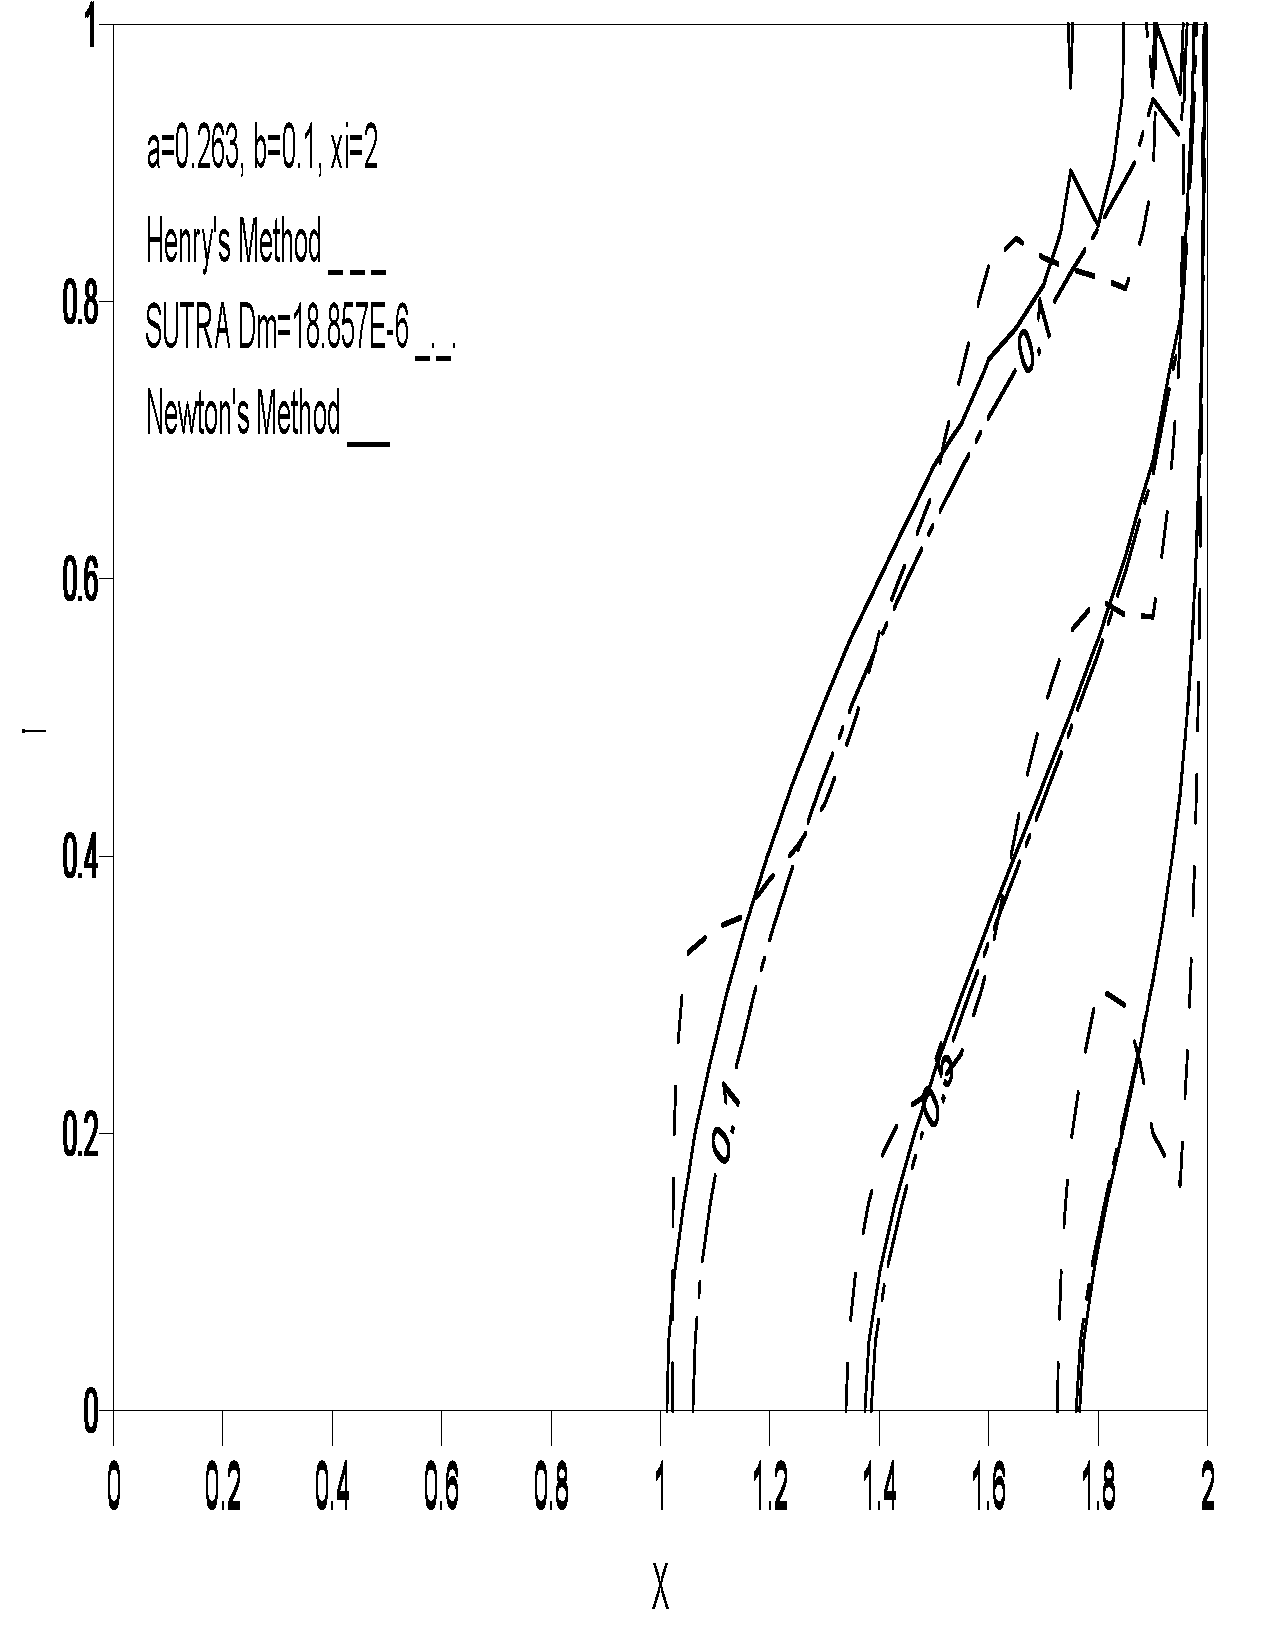
\includegraphics[totalheight=0.45 \textheight,viewport=3mm 4mm 205mm 292mm]
    {image2}
    \caption{Isochlor concentrations for $a = 0.263 \spbox{and} b =
    0.1$} \label{fig:b10-1}
\end{figure}

The second comparison ( \autoref{fig:b5x10-2}) used a value of 0.05 for $b$, and as one
can see an increase in instabilities in the upper 20\% of the solution domain resulted. As for
Henry's Method, instabilities were so great that the 0.1 isochlor contour shows up near $x=0.2
\text{ m} $. Once again the 0.9 isochlor contours for Newton's Method and SUTRA match very well, and
so does the 0.5 isochlors, but the 0.1 isochlor contours differ by a noticeable amount in their
position. Again it appears that as the concentration decreases from 0.9 to 0.1 the isochlor contours
begin to differ by greater amounts. As one can see from \autoref{fig:b5x10-5}, Newton's
Method and SUTRA do not agree as well as that of the previous comparison for $b=0.1$.

\begin{figure}[htp]
    \centering
    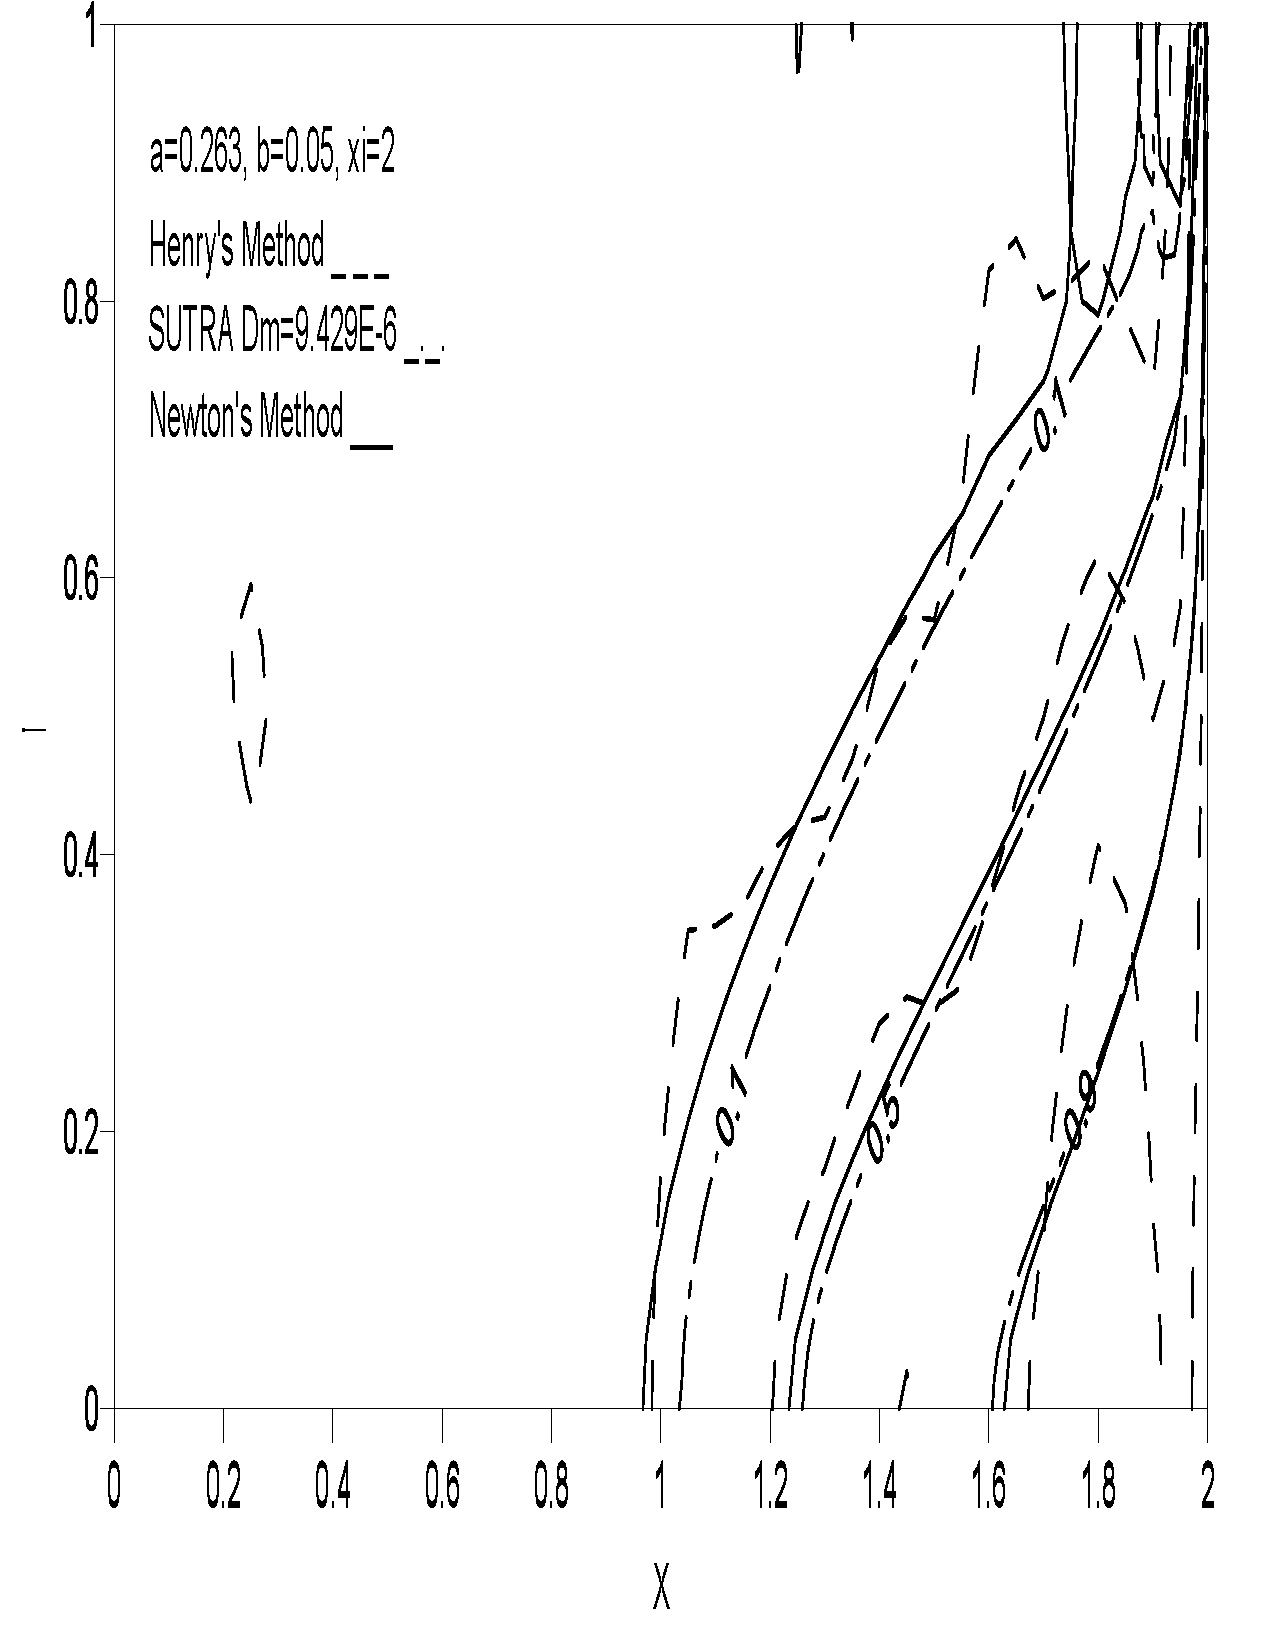
\includegraphics[totalheight=0.45 \textheight,viewport=3mm 4mm 205mm 292mm]
    {image3}
    \caption{Isochlor concentrations fo $a = 0.263 \spbox{and} b =
    0.05$} \label{fig:b5x10-2}
\end{figure}

The third comparison ( \autoref{fig:b6x10-3}), for which $b=6\times 10^{-3} $, resulted
in instabilities that created negative and 0.1 isochlors across the entire upper 20\% of the
solution domain for Newton's Method. Similar instabilities can be seen in the SUTRA solution for 231
nodes. One can see in the upper right hand corner the similar pattern that is also present in the
Newton's Method. The resulting 0.1 and 0.5 isochlors no longer match well.  However the 0.9 isochlor
is still very close. But, as one can see the lower values of $b$ create greater and greater
instabilities in the upper 20\% of the solution domain. These instabilities then further degrade the
accuracy of the isochlor contours in the lower 80\% of the solution domain. It is likely that a
larger number of Fourier coefficients could correct these problems, but due to a lack of computing
power and time this was unable to be checked. Henry's Method is not represented in this comparison,
due to the inability of this method to converge for values of $b$ lower than 0.05. It is believed
that the use of more Fourier coefficients would result in better agreement between SUTRA and Henry's
Semi-Analytic Solution.

\begin{figure}[htp]
    \centering
    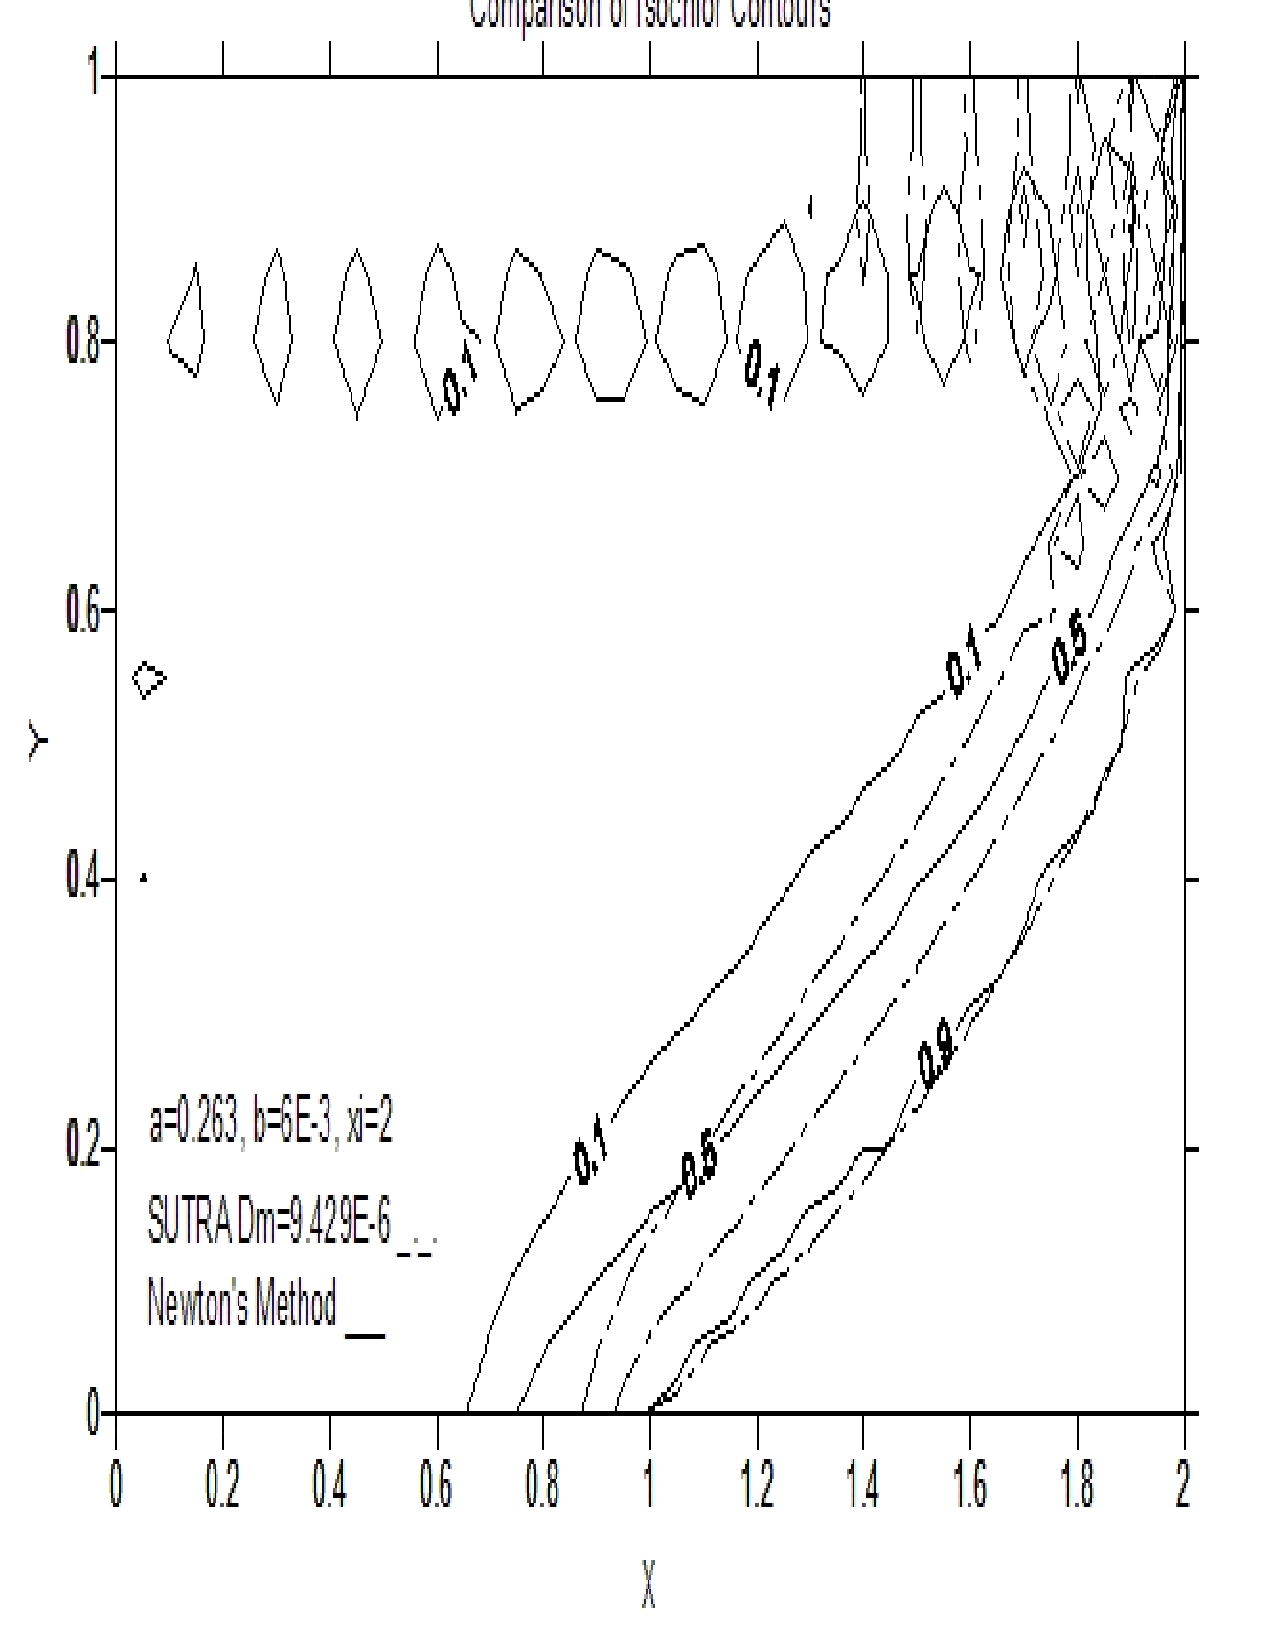
\includegraphics[totalheight=0.45\textheight,viewport=3mm 4mm 205mm 292mm]{image4}
    \caption{Isochlor concentrations for $a = 0.263 \spbox{and} b = 6 \times
    10^{-3}$} \label{fig:b6x10-3}
\end{figure}


\section{Conclusions}
Using Newton's Method to evaluate Henry's problem results in the ability to use a greater number of
Fourier coefficients than that of Henry's Method. This allows for an increase in the accuracy of the
solution. The increase in solution accuracy further allows for simulations of narrower zones of
dispersion (small values of $b$). The lower values of $b$ correspond to lower amounts of dispersion,
and therefore address the concerns stated by Voss and Souza \cite{Voss}, in which they say,
``because of the unrealistic large amount of dispersion introduced in the solution by the constant
total dispersion coefficient, this test does not check whether a model is consistent or whether it
accurately represents density driven flows, nor does it check whether a model can represent field
situations with relatively narrow transition zones.'' 

It appears that a further increase in the total number of Fourier coefficients may be necessary to
address the issue of instabilities created when evaluating Henry's Problem for low values of b. Due
to time constraints the number of Fourier coefficients for this analysis was limited to 1860
coefficients. It is believed that the number of Fourier coefficients to quell the instabilities may
be in excess of 5100 coefficients. The majority of time needed for each iteration was in the
evaluation of the Jacobian matrix $D\Phi $. A quicker algorithm for calculating the total derivative
function may be able to be developed, and therefore it may be possible to evaluate Henry's Problem
using a greater number of Fourier coefficients in a more timely fashion.

In addition to developing a more efficient algorithm for the total derivative function, it might be
necessary to use a more robust numerical method than that of Newton's Method. If a more robust
numerical method is used it may be able to address the instabilities in the upper 20\% of the
solution domain, without a further increase in the number of Fourier coefficients used in the
evaluation of Henry's Problem. It is clear that using Newton's Method over that of Henry's Method
increases the stability of Henry's Problem. This increase in stability resulted in the ability to
use a larger number of Fourier coefficients, and therefore an increase in the accuracy of the
solution. The increase in solution accuracy then resulted in the ability to evaluate Henry's Problem
for values of $b<0.05$. Using an even more robust numerical method may have similar results.


\bibliographystyle{plain}
\bibliography{Henry}

\end{document}
